\documentclass[10pt, aspectratio=43]{beamer}

\usetheme[secheader]{Madrid}
\usecolortheme{whale}
\usefonttheme{serif}
\bibliographystyle{plain}

\usepackage[utf8]{inputenc}
\usepackage[french]{babel}
\usepackage[T1]{fontenc}
\usepackage{graphicx}
\usepackage{tikz}
\usepackage{rotating}
%\usepackage{caption}
%\usepackage{textcomp}

\usetikzlibrary{graphs}

\setbeamerfont{title}{size=\Large}
\setbeamerfont{author}{size=\large}
\setbeamerfont{institute}{size=\normalsize}
\setbeamerfont{date}{size=\normalsize}
\setbeamertemplate{caption}[numbered]
\graphicspath{ {./} }
%\captionsetup[figure]{font=scriptsize, justification=centering,labelfont=bf,labelformat=empty}

\title[Résolution de puzzle]{Résolution numérique de puzzle}
\subtitle{Travail d'Initiative Personnelle Encadré - Transition, transformation, conversion}
\author[C. PERIER]{\textbf{Cyriaque PERIER}\vspace{-0.5em}}
\institute[\textbf{N\textdegree 10002}]{Candidat N\textdegree 10002 \vspace{-0.5em}}
\date{2024 - 2025}

\begin{document}

	\begin{frame}

		\vspace{-5em}

		\titlepage
		\begin{center}

			\vspace{-4em}
			Filière MP - Option Informatique
			%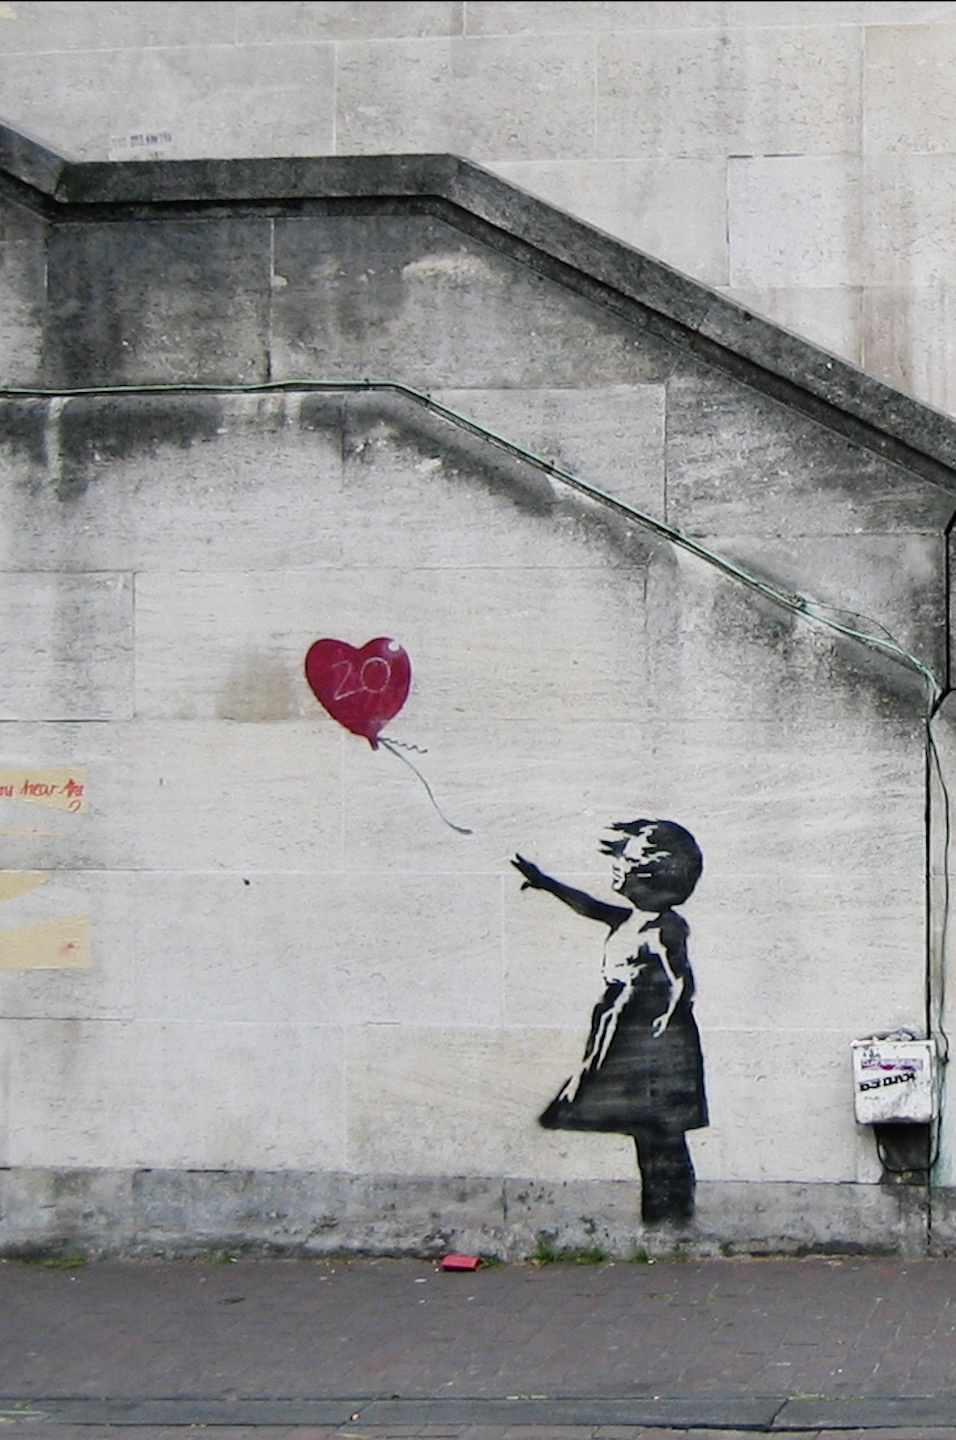
\includegraphics[width=\linewidth, height=0.40\textheight, keepaspectratio]{../Images/GirlwithBalloon}

		\end{center}

		\vspace{-10em}
		\hfill
		\begin{turn}{-90}\fontsize{2.5}{4}\selectfont Version du \today\end{turn}

	\end{frame}

	\section{Introduction}
	\begin{frame}{Le problème des puzzles}
		\centering
		5 Octobre 2018 - Destruction du tableau \underline{Girl with Balloon} de \emph{Banksy}
		\vspace{10pt}

		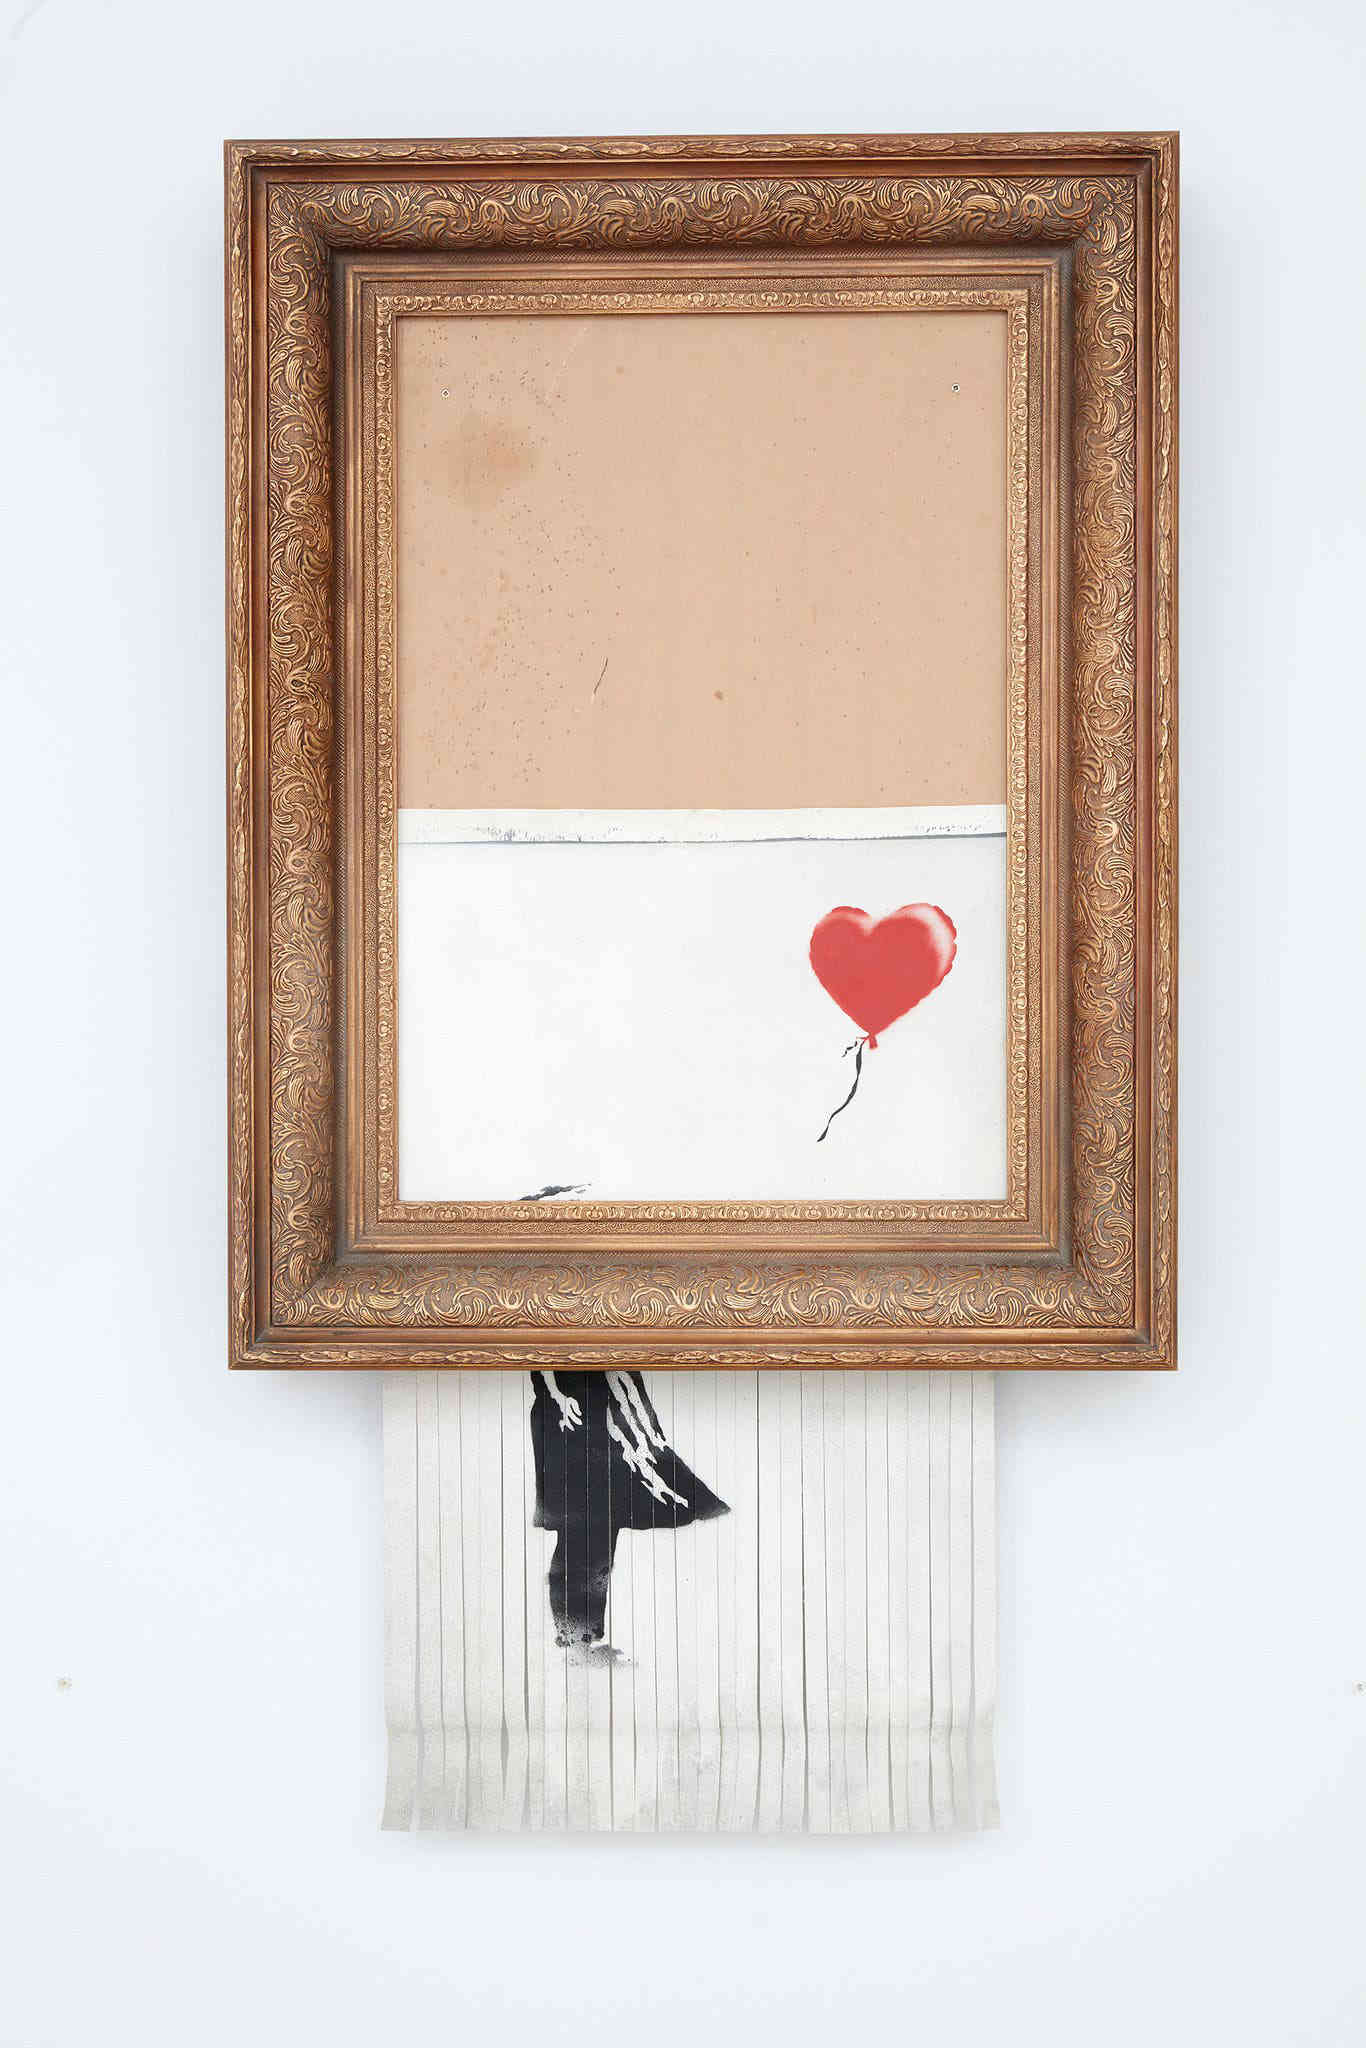
\includegraphics[width=\linewidth, height=0.60\textheight, keepaspectratio]{../Images/banksy2}

		\footnotesize Source : \underline{The New York Times}
	\end{frame}
	\begin{frame}{Intérêt d'une solution de ce problème}
		\centering
		16 Millions de pages déchiquetées par la \emph{Stasi}
		\vspace{10pt}

		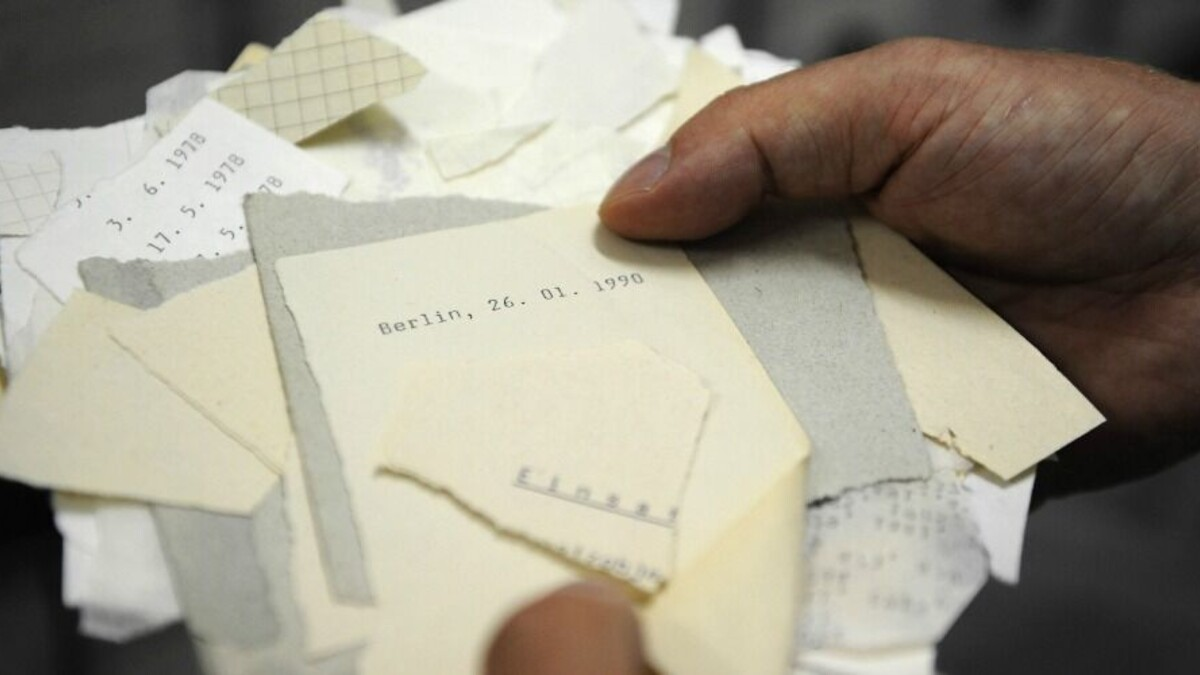
\includegraphics[width=\linewidth, height=0.60\textheight, keepaspectratio]{../Images/stasi}

		\footnotesize Source : \underline{Agence France-Presse}
	\end{frame}
	\begin{frame}{Problématique}
		\centering
		\Large \textbf{Comment résoudre numériquement des puzzles d'image et reconstituer leur agencement ?}
	\end{frame}
	\begin{frame}{Table des matières}

		
		\tableofcontents
		

	\end{frame}
	\section{Cas général}

	\begin{frame}{Table des matières}

		
		\tableofcontents[currentsection]
		

	\end{frame}

	\subsection{Distance entre deux fragments}
	\begin{frame}{Distance entre deux fragments}

		
		\centering
		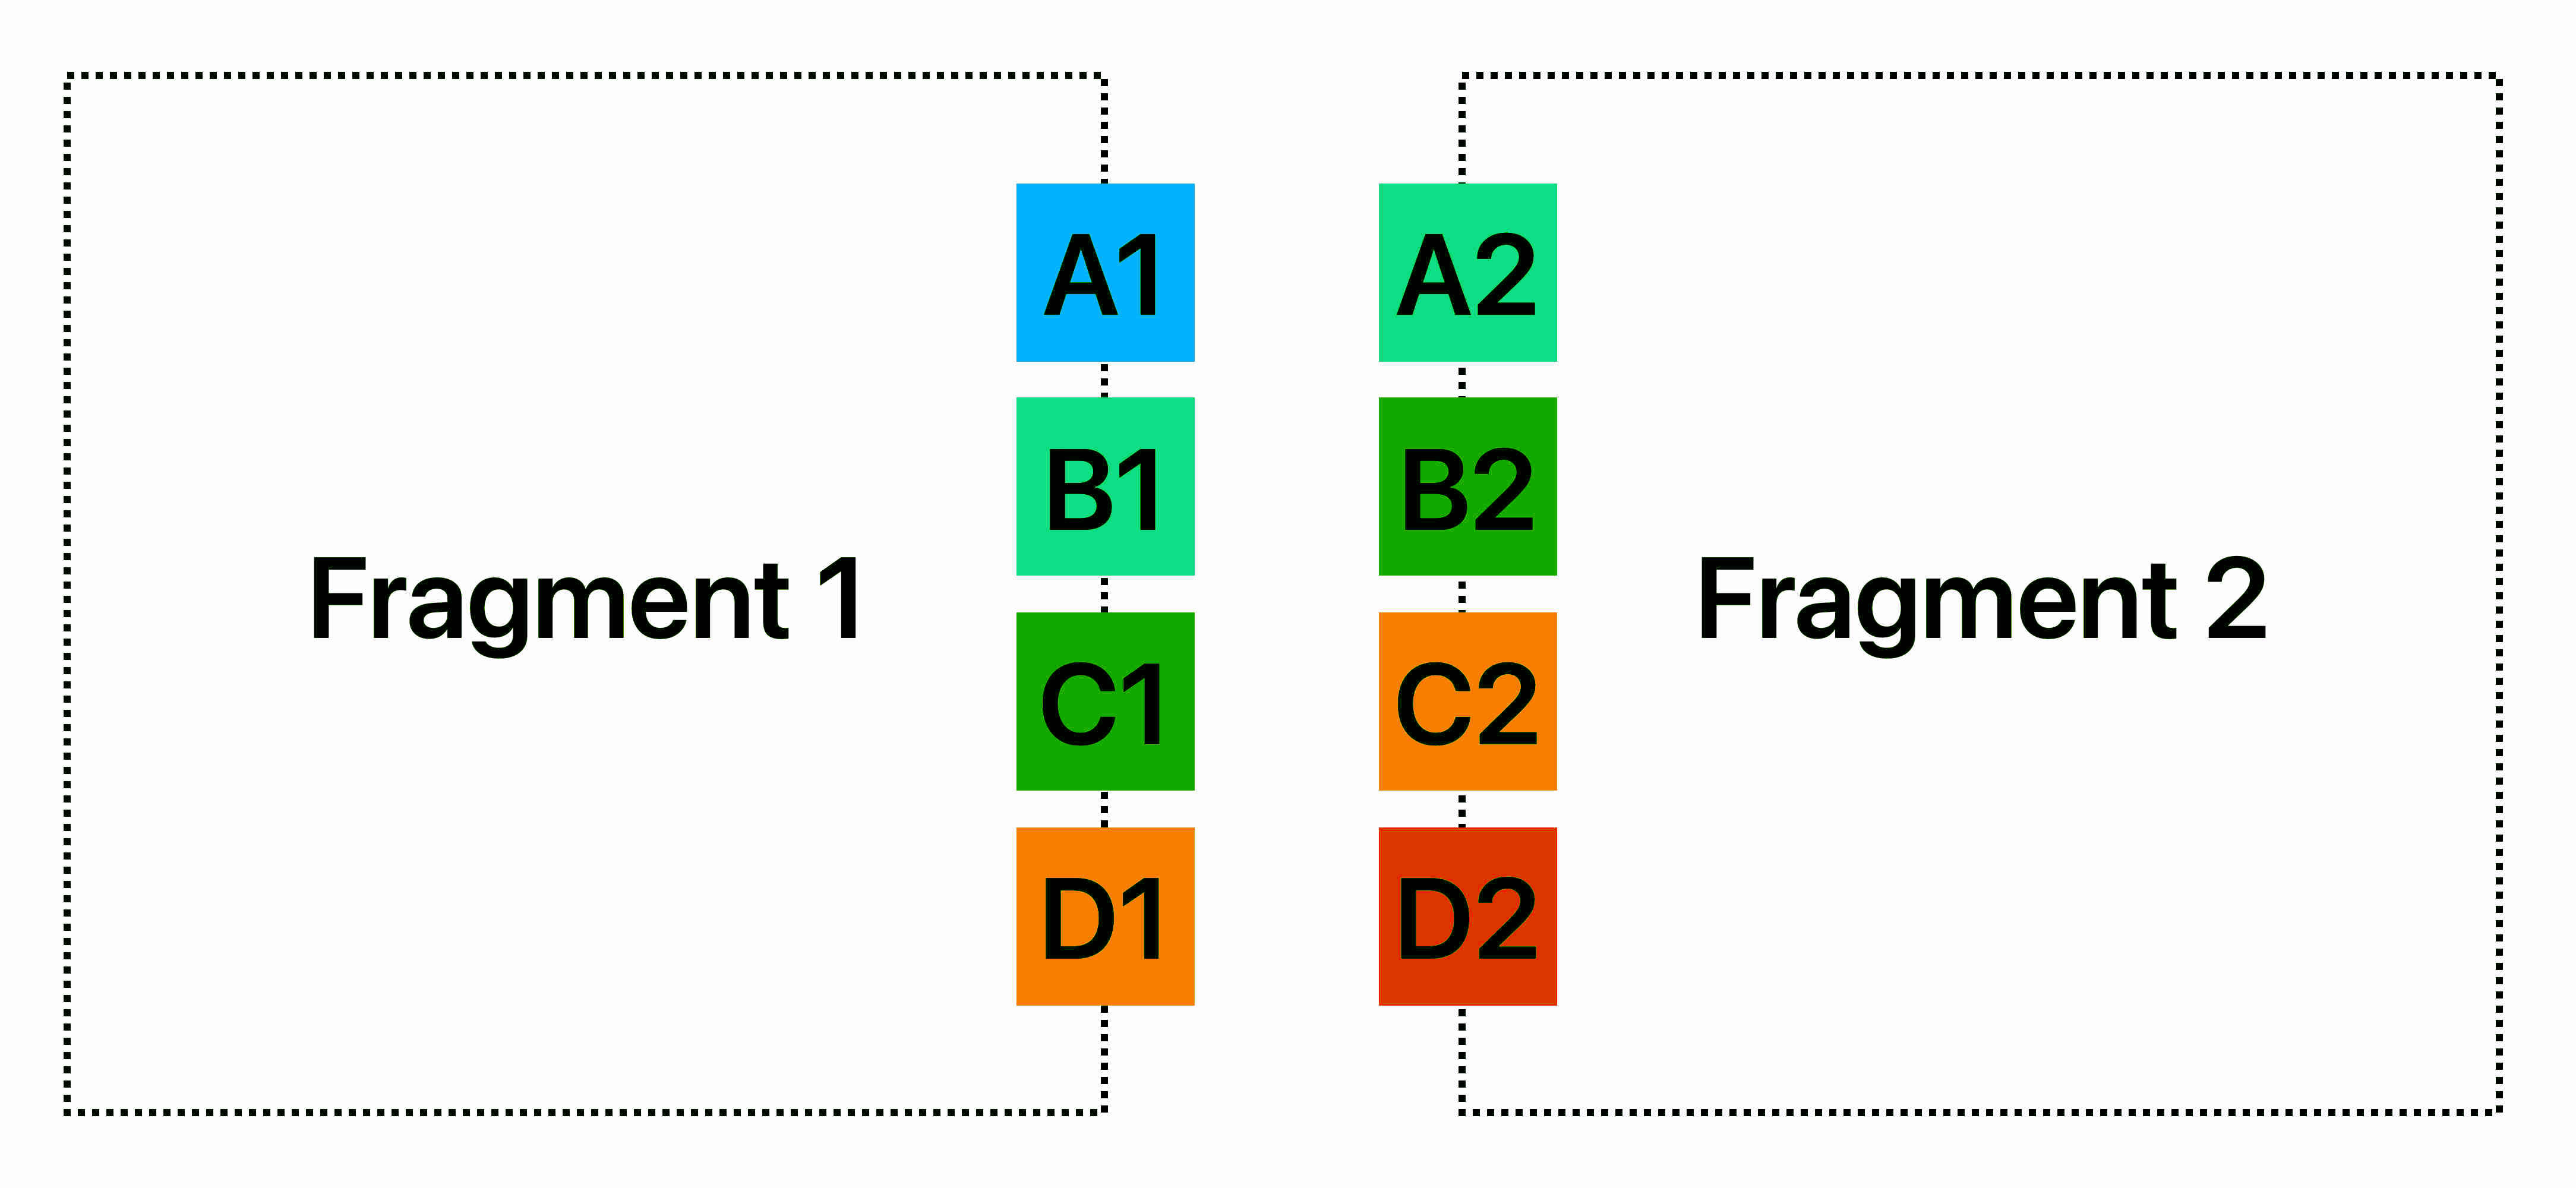
\includegraphics[width=\linewidth, height=0.9\textheight, keepaspectratio]{../Images/illustration_norme}
		\[ \centering d = |A1 - A2| + ... + |D1 - D2| \]
		

	\end{frame}

	\subsection{Résolution par algorithme glouton}
	\begin{frame}{Résolution par algorithme glouton}
		\centering
	    \begin{minipage}[b]{0.40\textwidth}
	        \centering
	        \vspace{0pt}
	        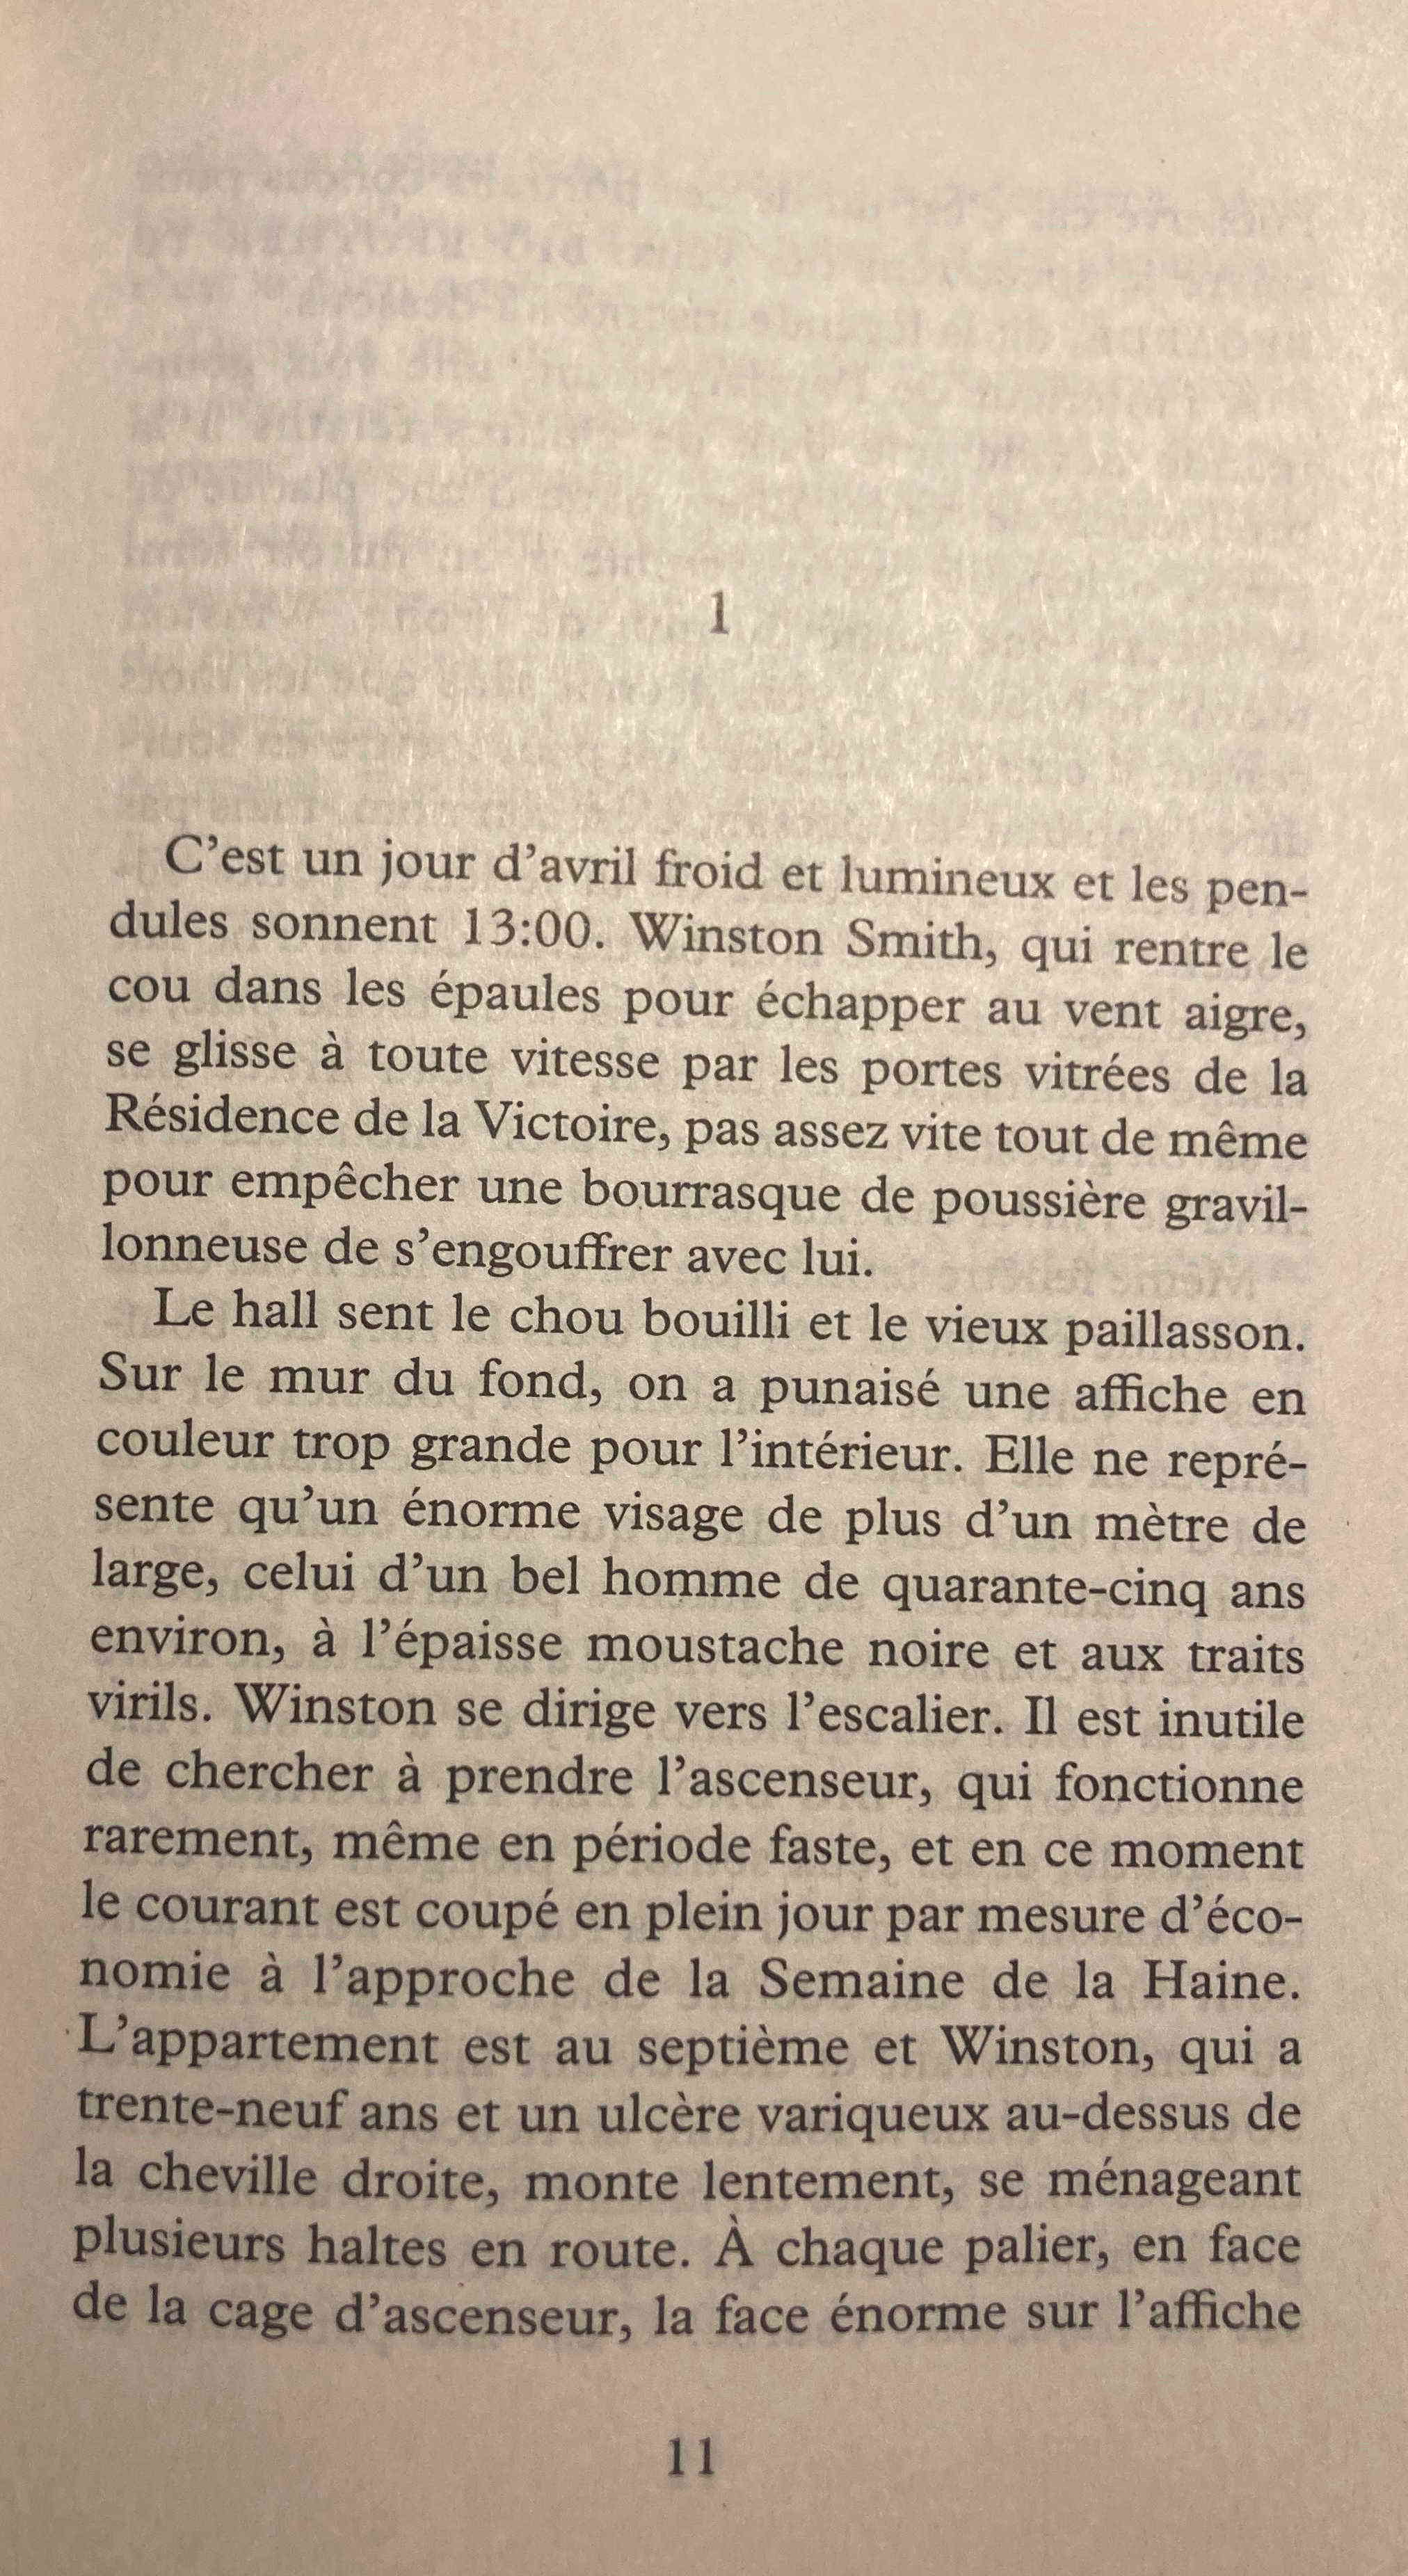
\includegraphics[width=\linewidth, height=0.7\textheight, keepaspectratio]{../Images/1984_cpr} \\
	        Poids de la solution : 5 040 074
	    \end{minipage} 
	    \hspace{20pt}
	    \begin{minipage}[b]{0.40\textwidth}
	        \centering
	        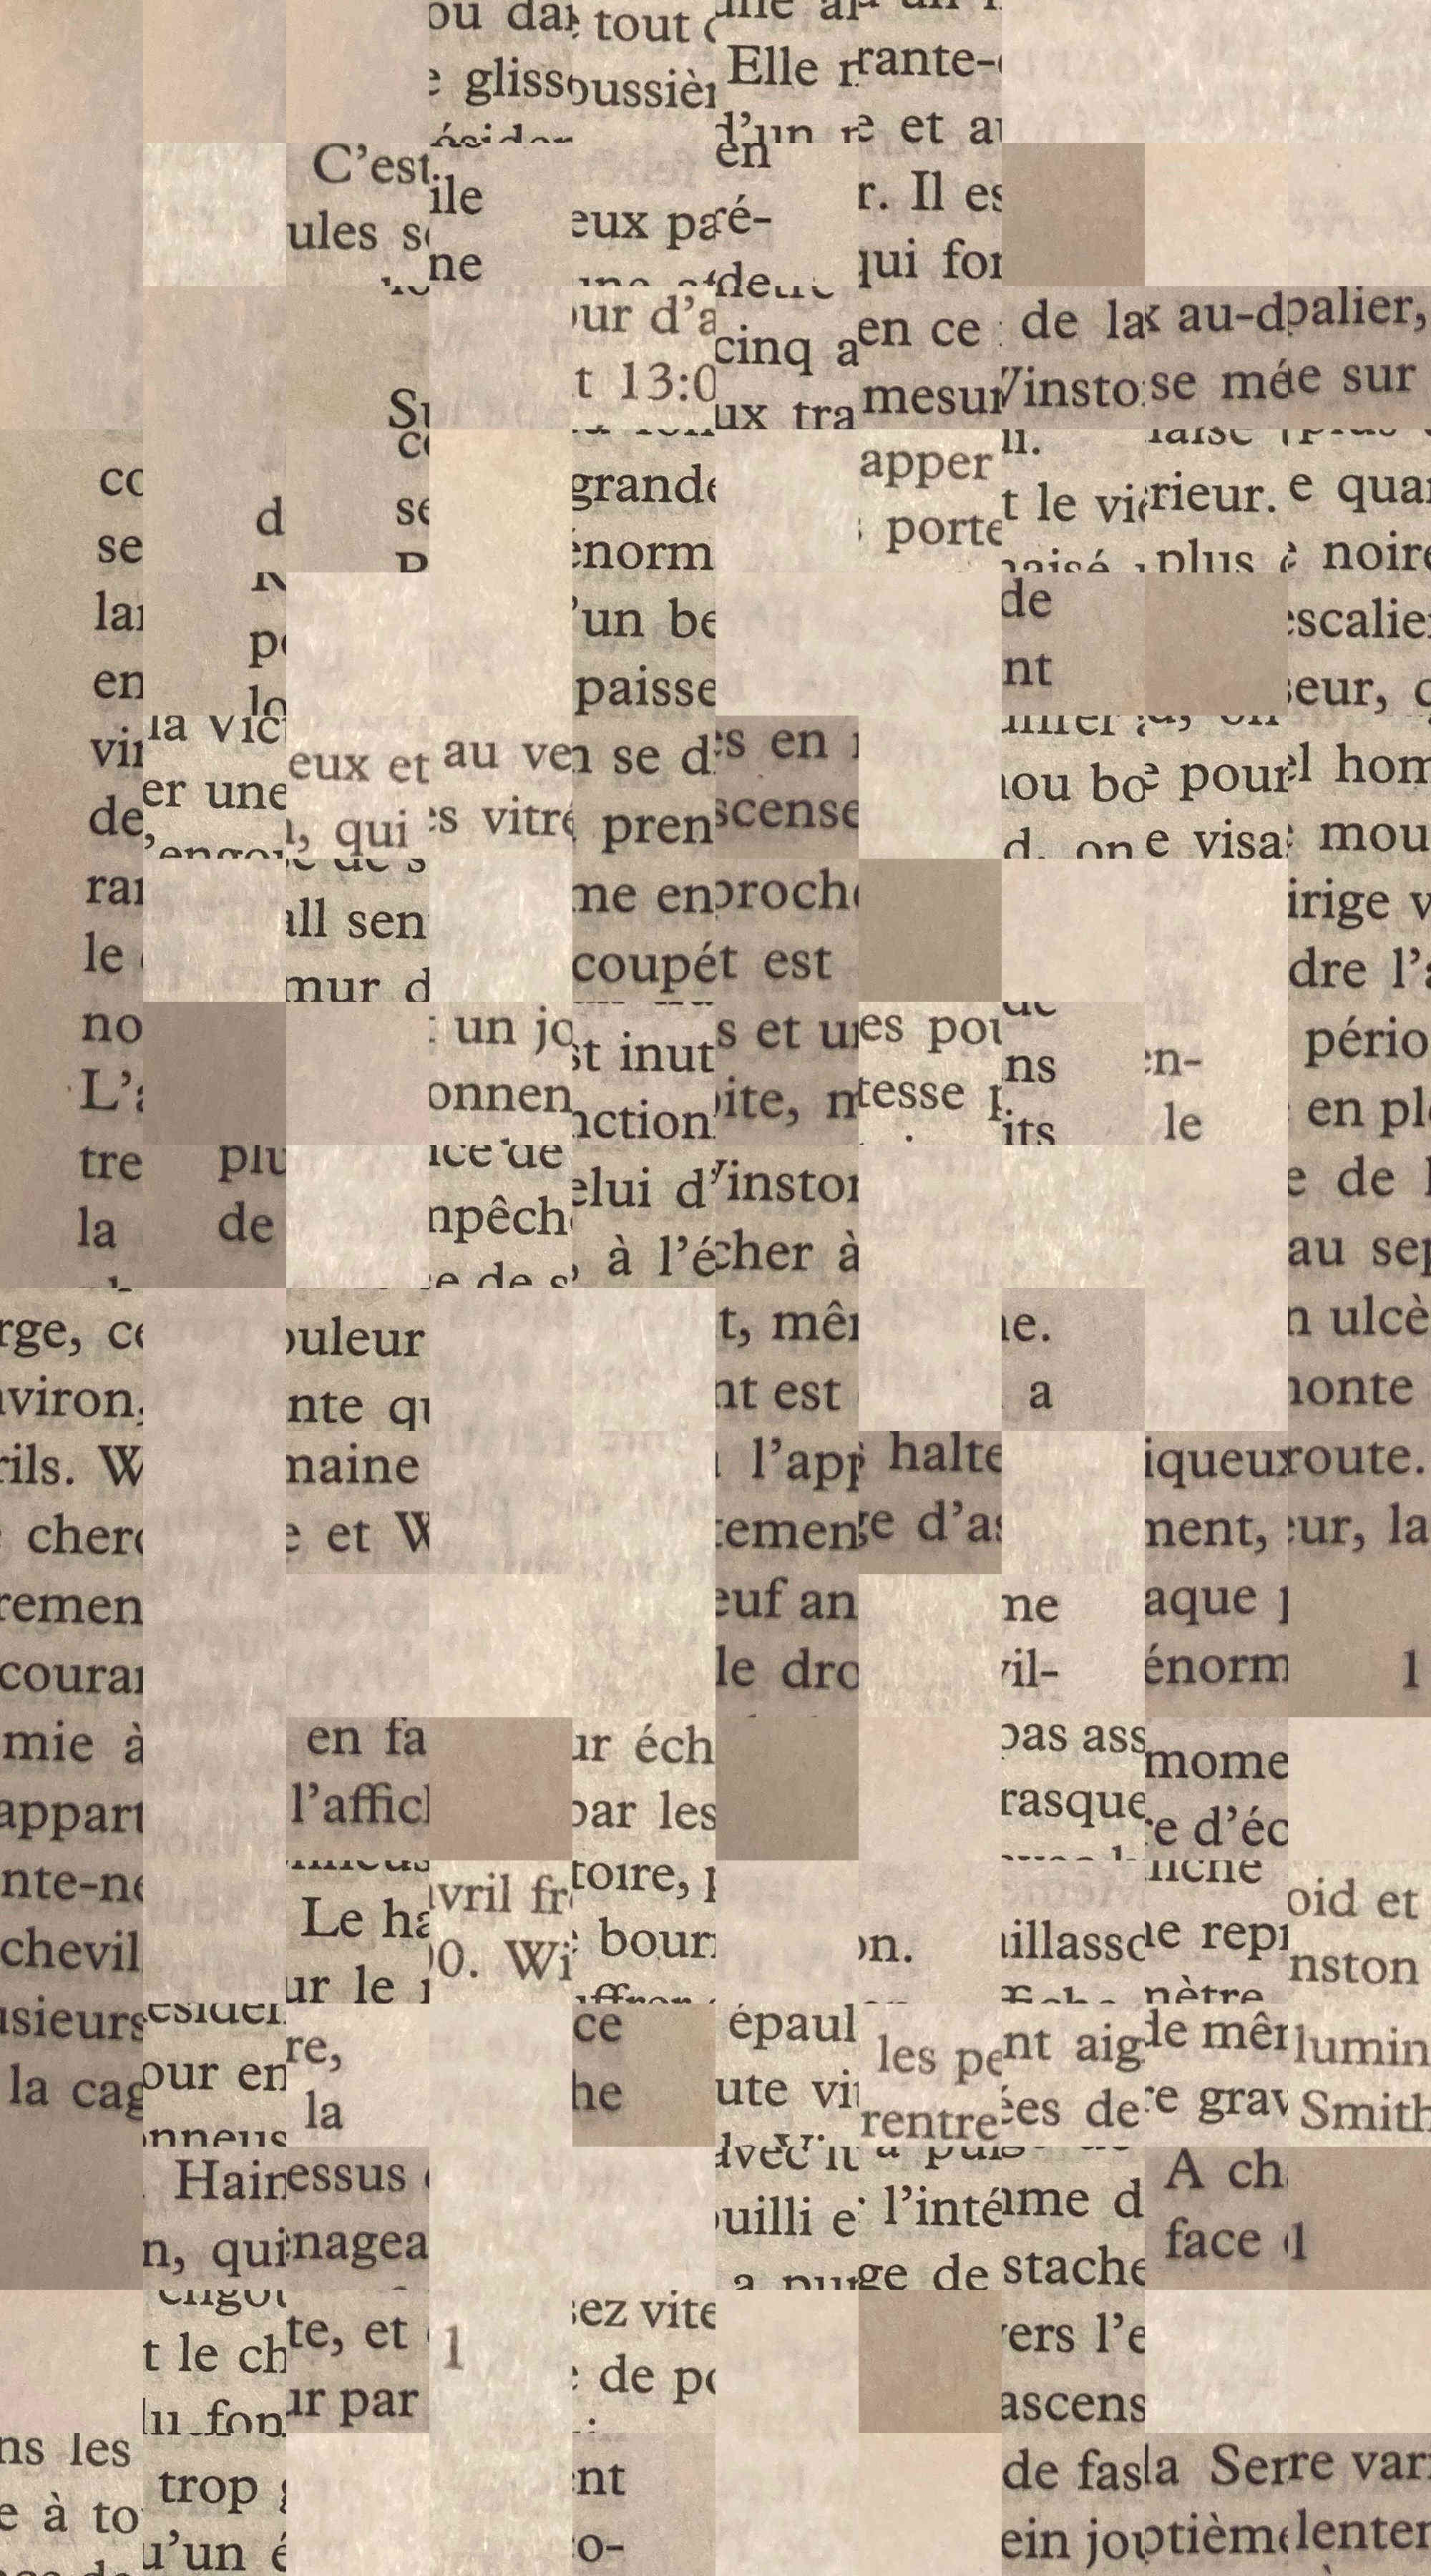
\includegraphics[width=\linewidth, height=0.7\textheight, keepaspectratio]{../Images/1984_bestgreedy_cpr} \\
	        Poids de la solution : 4 084 977
	    \end{minipage}

	    \footnotesize Source : \underline{1984}, G. Orwell
	\end{frame}

	\subsection{La difficulté de trouver une distance}
	\begin{frame}{La difficulté de trouver une distance}
		\centering
		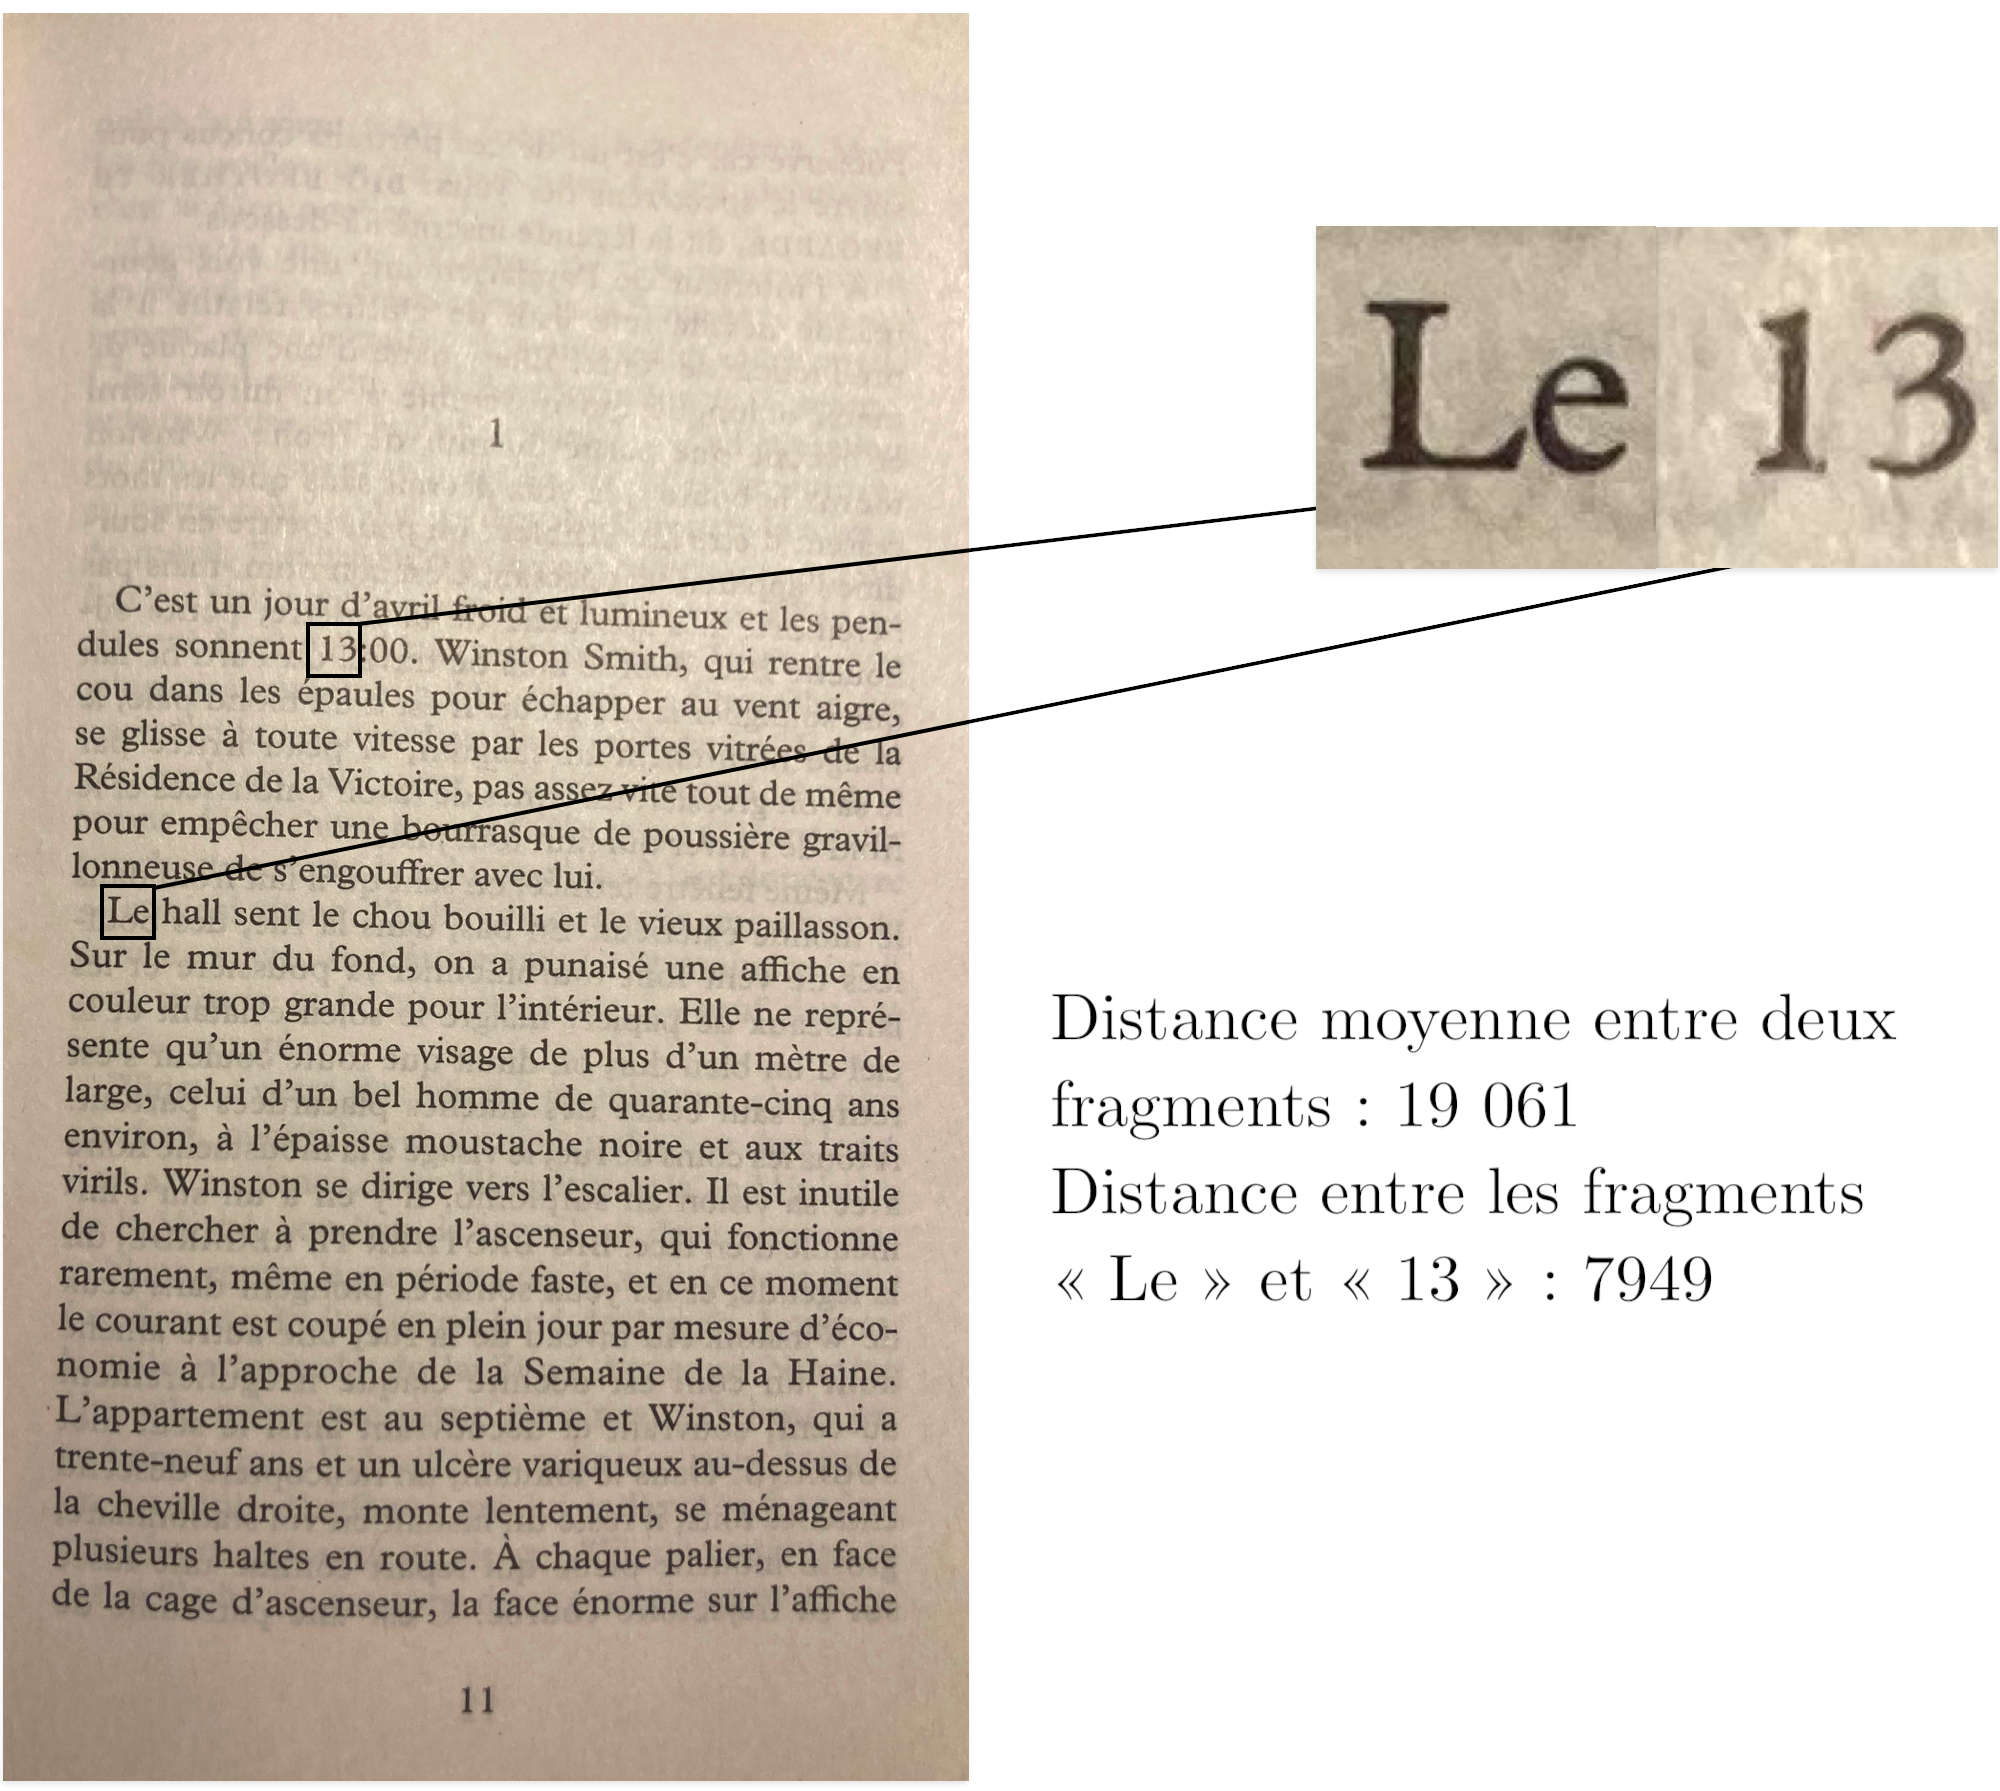
\includegraphics[width=\linewidth, height=0.8\textheight, keepaspectratio]{../Images/norme}
	\end{frame}

	\section[Cas particulier]{Cas particulier de l'image basse définition de la solution}

		\begin{frame}{Table des matières}

			
			\tableofcontents[currentsection]
			

		\end{frame}

	\subsection[Présentation]{Présentation du cas particulier}
	\begin{frame}{Présentation du cas particulier}
		\centering
		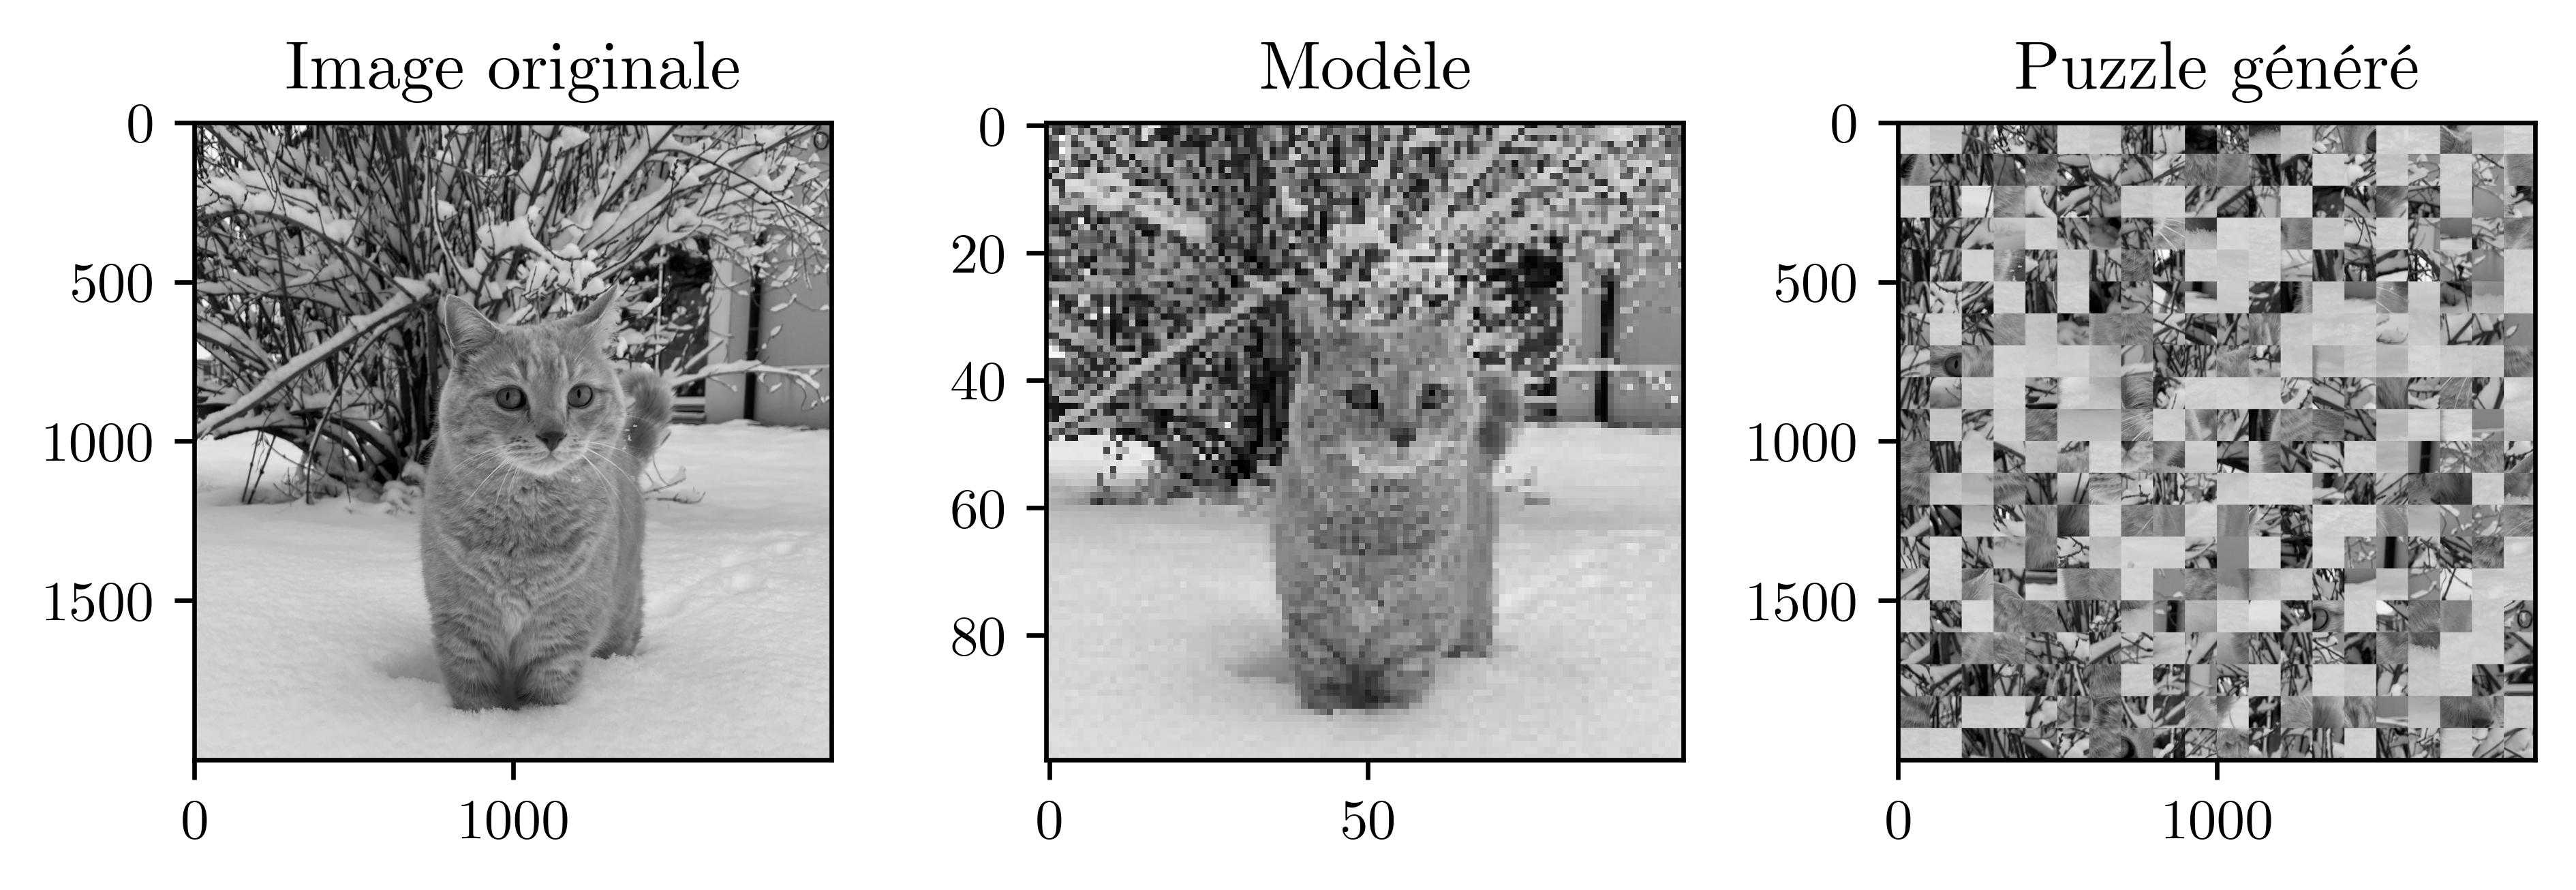
\includegraphics[width=\linewidth, height=0.9\textheight, keepaspectratio]{../Images/tigrou_pres}
	\end{frame}
	\subsection[Modélisation]{Modélisation du problème}
	\begin{frame}{Modélisation du problème}
		\centering
		\begin{tikzpicture}[every node/.style={circle, draw}, node distance=1.5cm and 2.5cm]

		  % Nodes A
		  \node (A1) at (0,3) {A1};
		  \node (A2) at (0,2) {A2};
		  \node (A3) at (0,1) {A3};
		  \node (A4) at (0,0) {A4};

		  % Nodes B
		  \node (B1) at (5,3) {B1};
		  \node (B2) at (5,2) {B2};
		  \node (B3) at (5,1) {B3};
		  \node (B4) at (5,0) {B4};

		  % Draw edges from A to B with labels
		  \foreach \i in {1,2,3,4} {
		    \foreach \j in {1,2,3,4} {
		      \draw (A\i) -- (B\j);
		    }
		  }

		\end{tikzpicture}
		\underline{Modélisation sous forme de graphe bipartie}
	\end{frame}
	\subsection[Résolution]{Résolution du problème}
	\begin{frame}{Résolution du problème}
		\centering
		\includegraphics[width=\linewidth, height=0.9\textheight, keepaspectratio]{../Images/stratégie_pattern_matching}
		\underline{Schéma de la stratégie de résolution}
	\end{frame}
	\subsection[Exemple]{Exemple de résolution}
	\begin{frame}{Exemple de résolution}
		\centering
		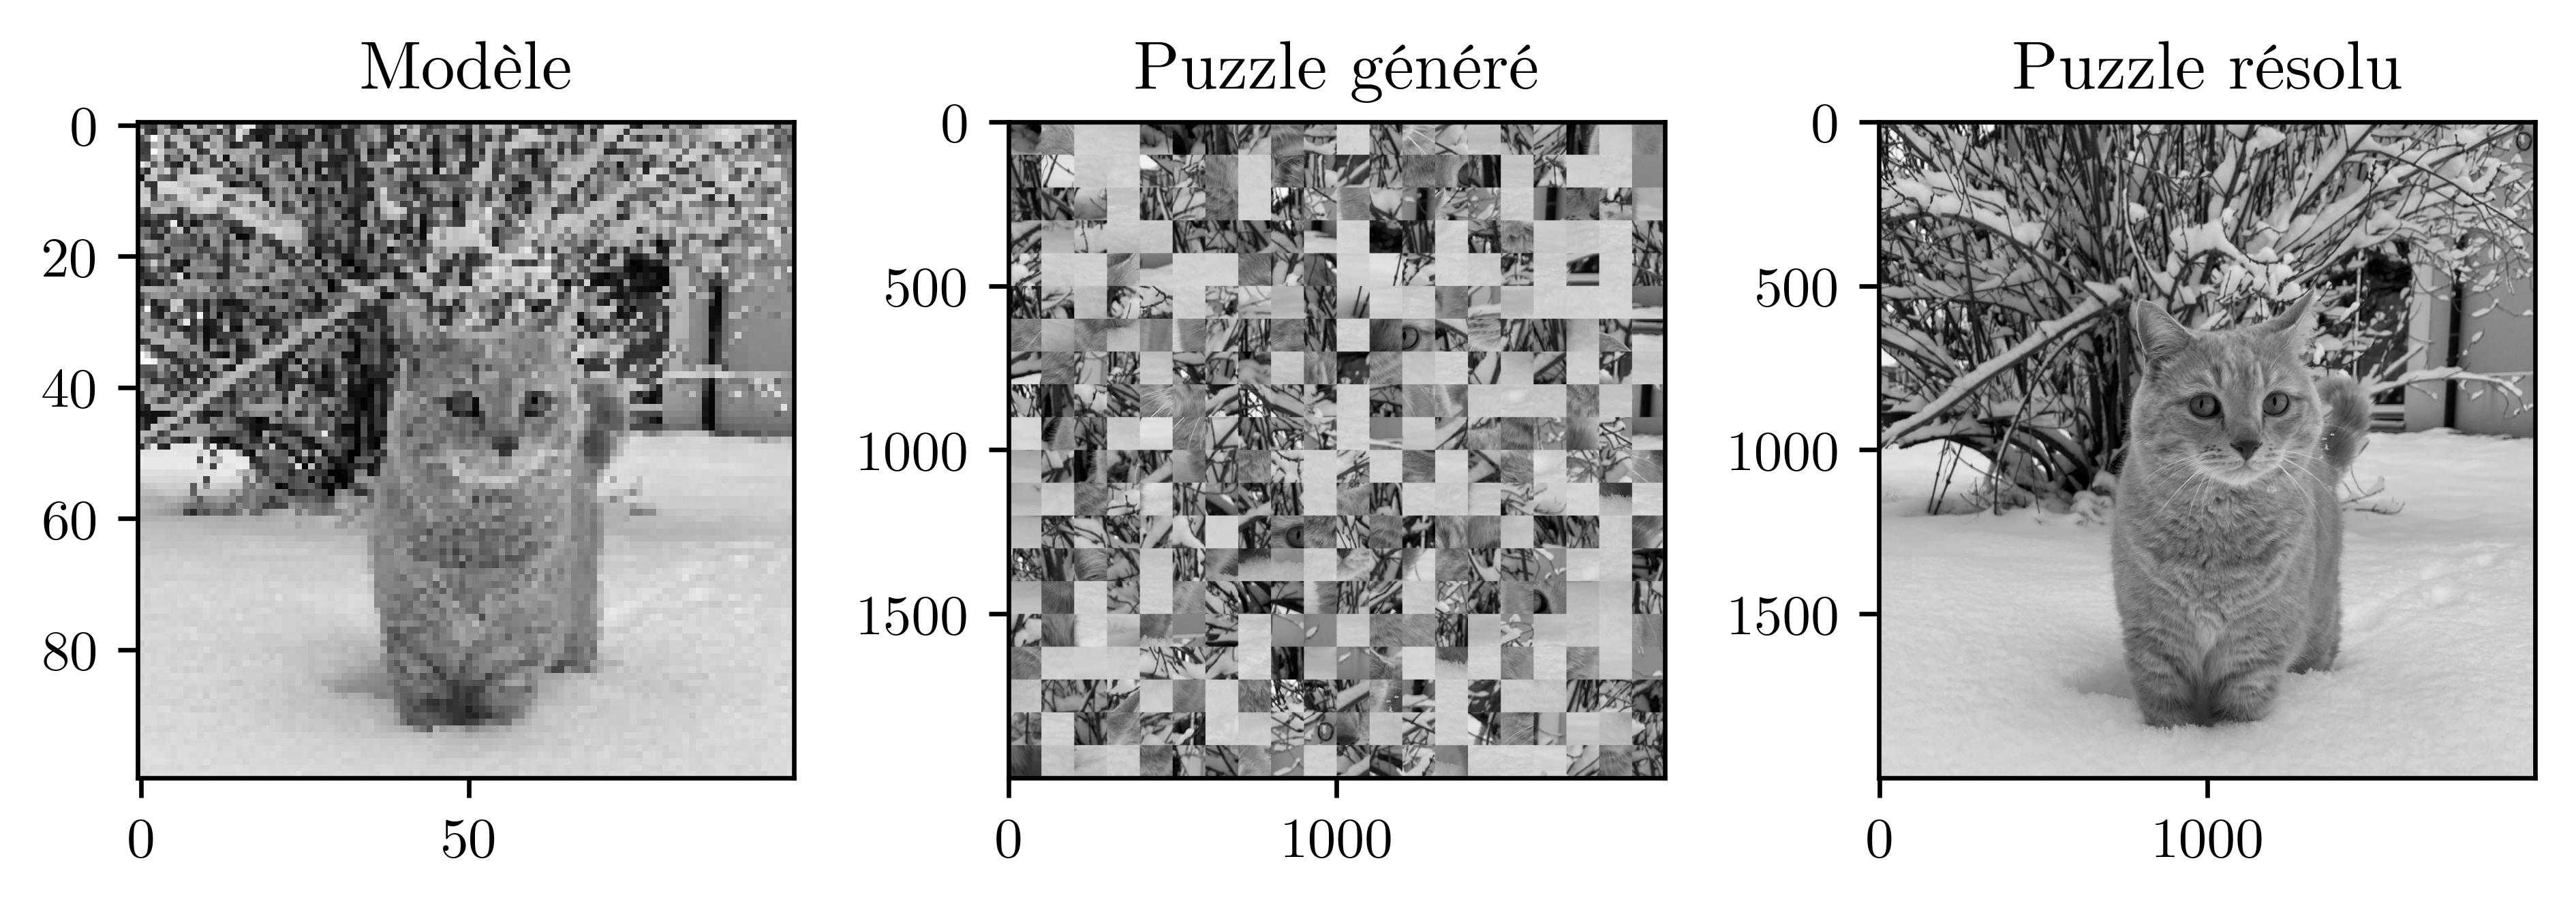
\includegraphics[width=\linewidth, height=0.9\textheight, keepaspectratio]{../Images/tigrou_exemple}
	\end{frame}

	\section[Tests]{Validation de la méthode par des tests}
	\begin{frame}{Table des matières}
		
		\tableofcontents[currentsection]
		
	\end{frame}
	\begin{frame}{Résultats des tests}
		\centering
		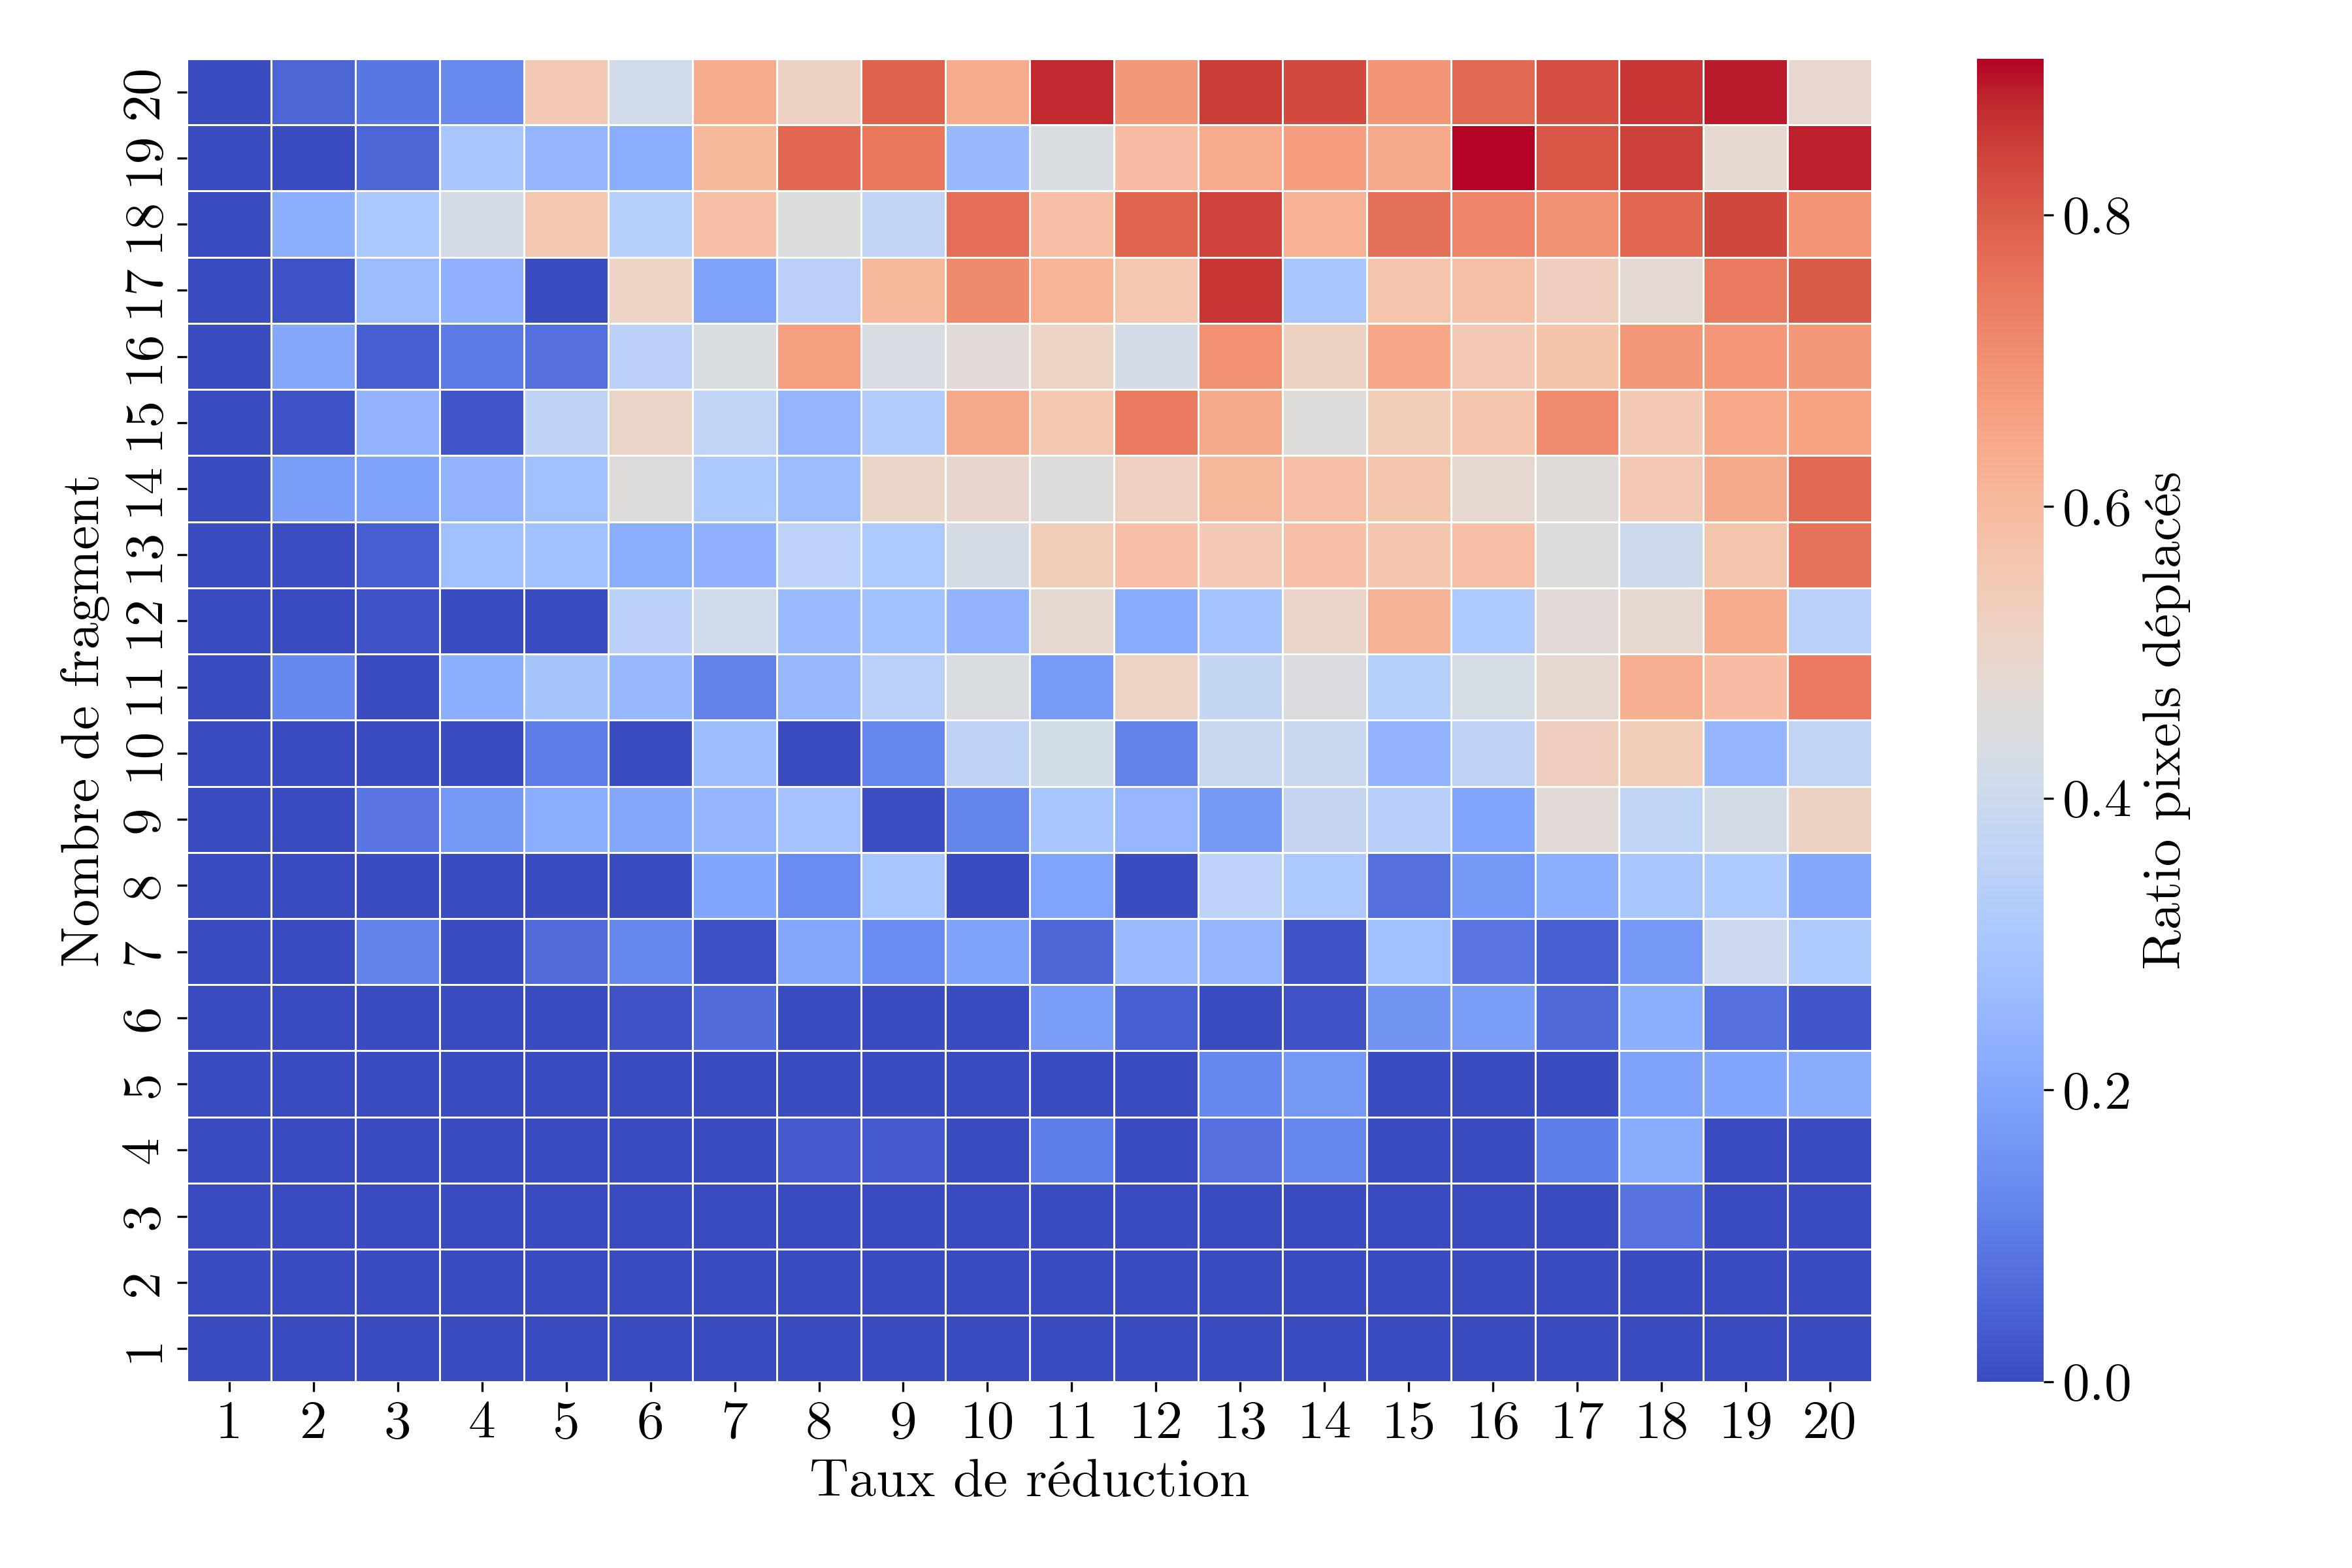
\includegraphics[width=\linewidth, height=0.8\textheight, keepaspectratio]{../Images/tests}
		\underline{Résultats des tests}
	\end{frame}

	\section{}

	\begin{frame}
		\centering
		\Large Merci pour votre attention.
	\end{frame}

	\section{Annexes}


	\begin{frame}{Annexe 1 - Taille des fragments basses définitions}
		\centering
		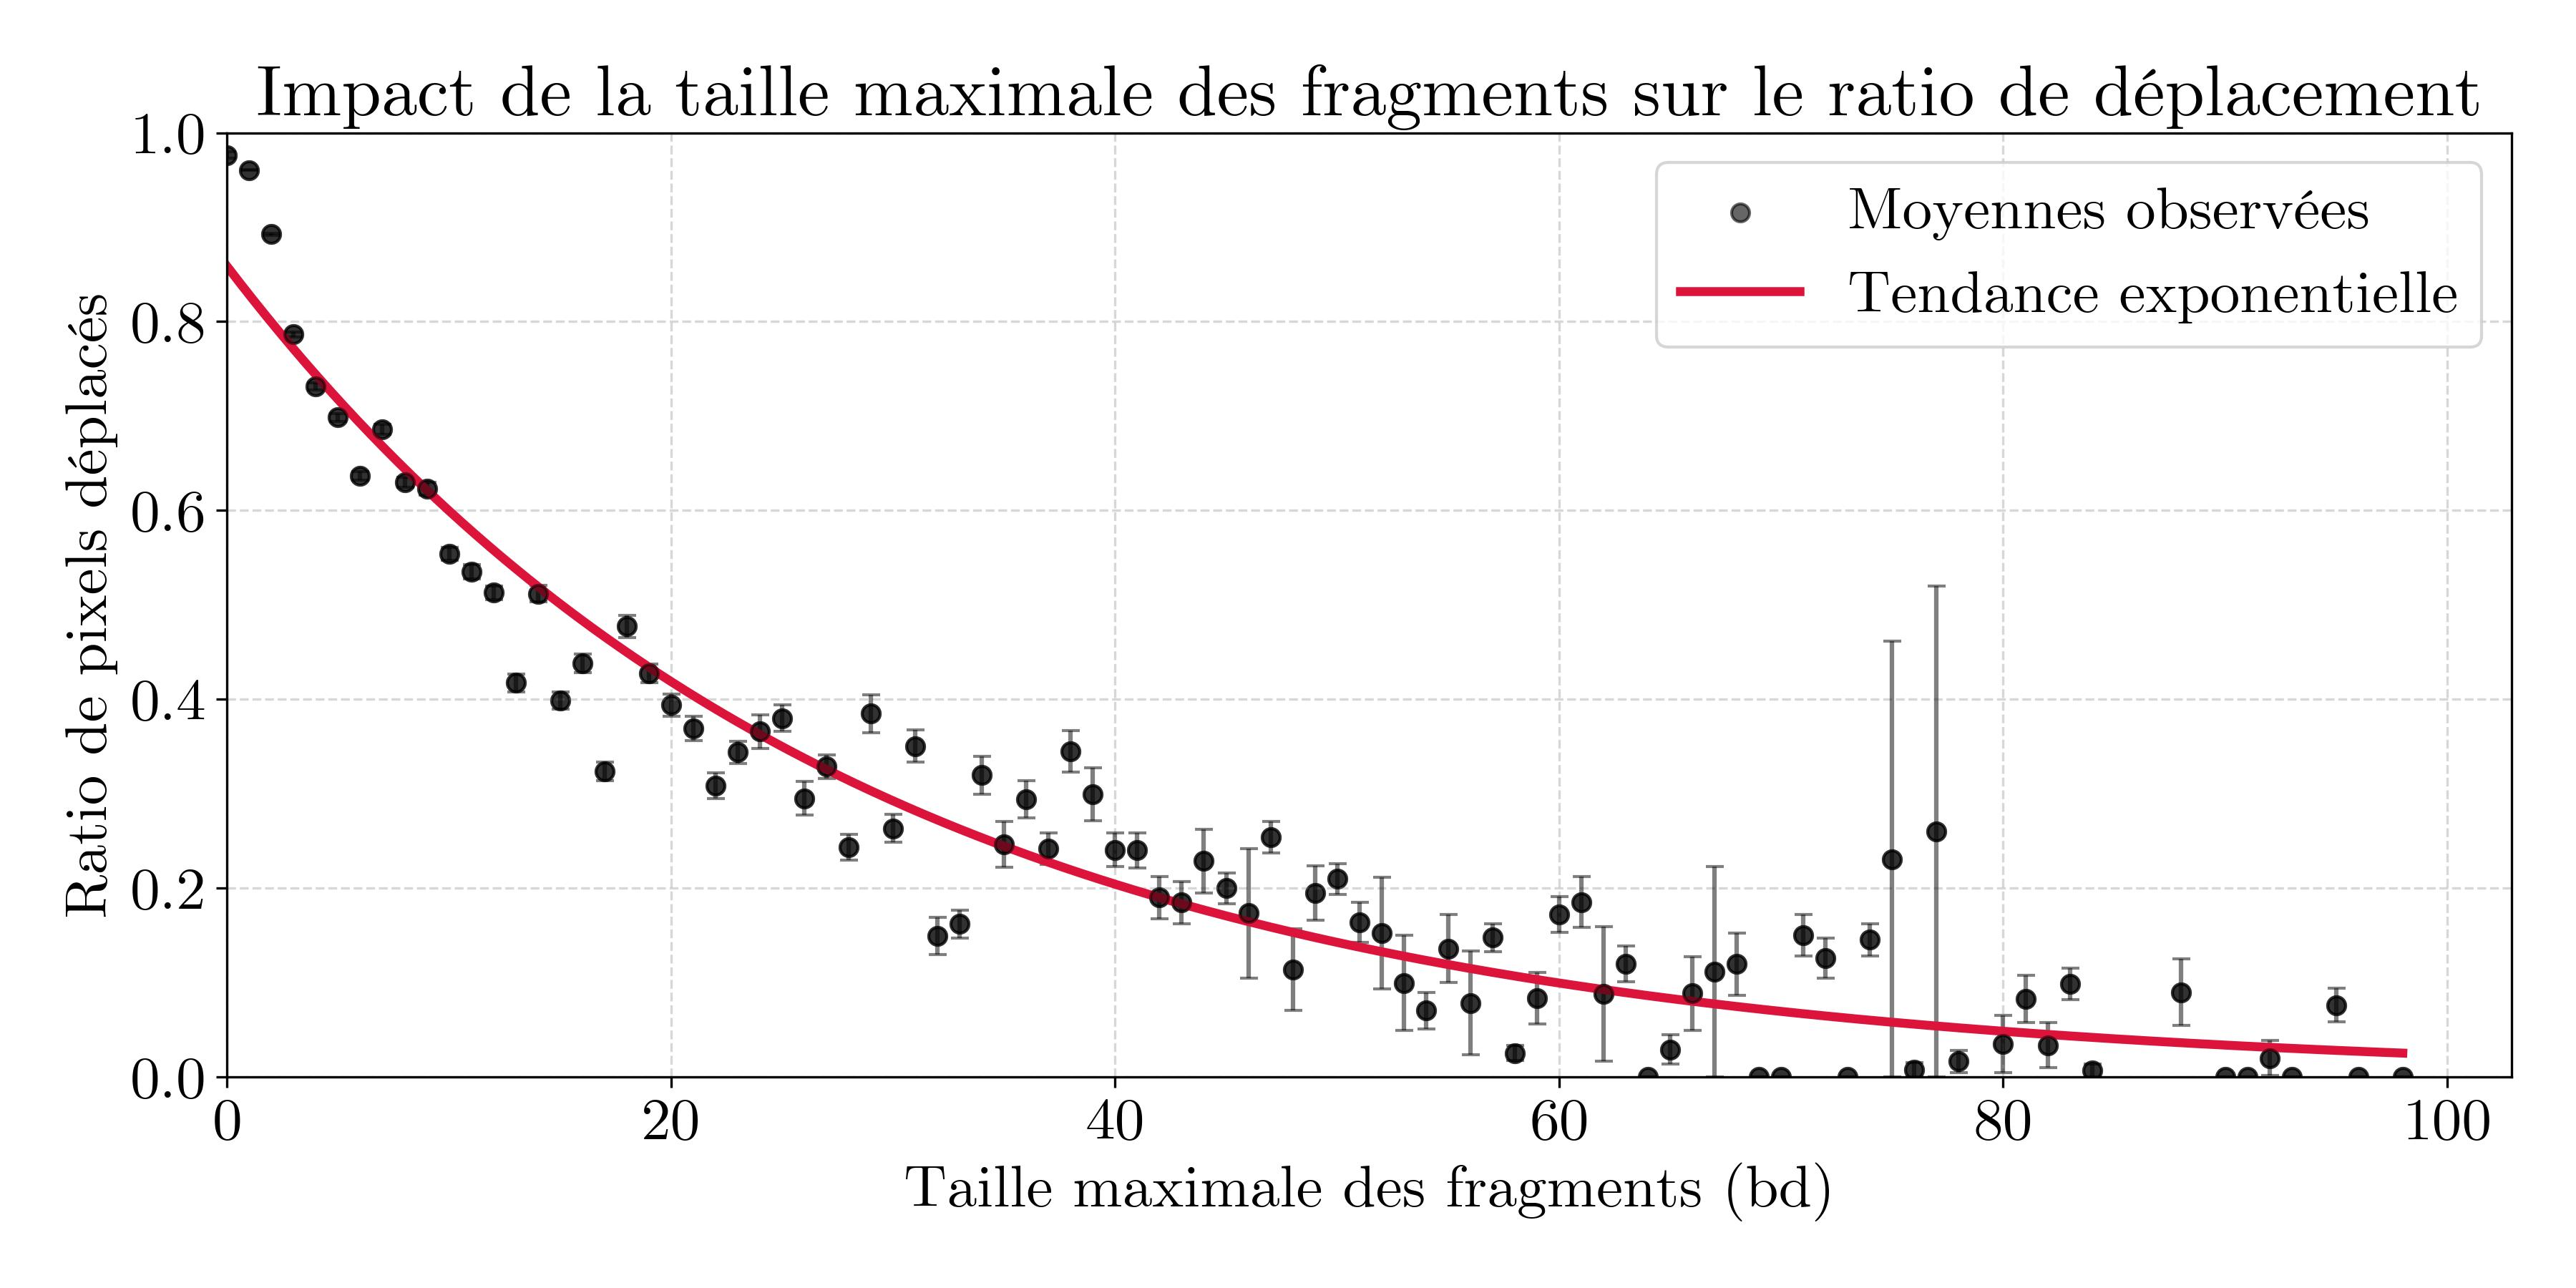
\includegraphics[width=\linewidth, height=0.8\textheight, keepaspectratio]{../Images/ratio_vs_maxfrag_tendance}
		\underline{Résultats des tests}
		\underline{Erreur en fonction de la taille des fragments basse définition}
	\end{frame}

	\begin{frame}{Annexe 2 - Distribution des distances}
		\centering
		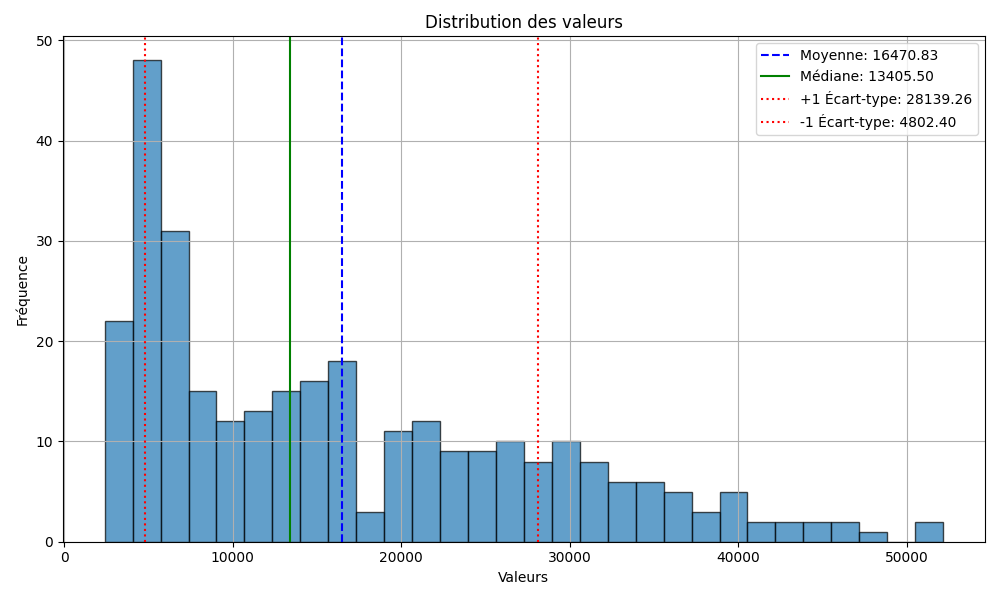
\includegraphics[width=\linewidth, height=0.8\textheight, keepaspectratio]{../Images/distribution_distances}
		\underline{Distribution des distances entre fragments}
	\end{frame}

	\begin{frame}{Annexe 3 - Exemple d'échec de résolution}
		\centering
		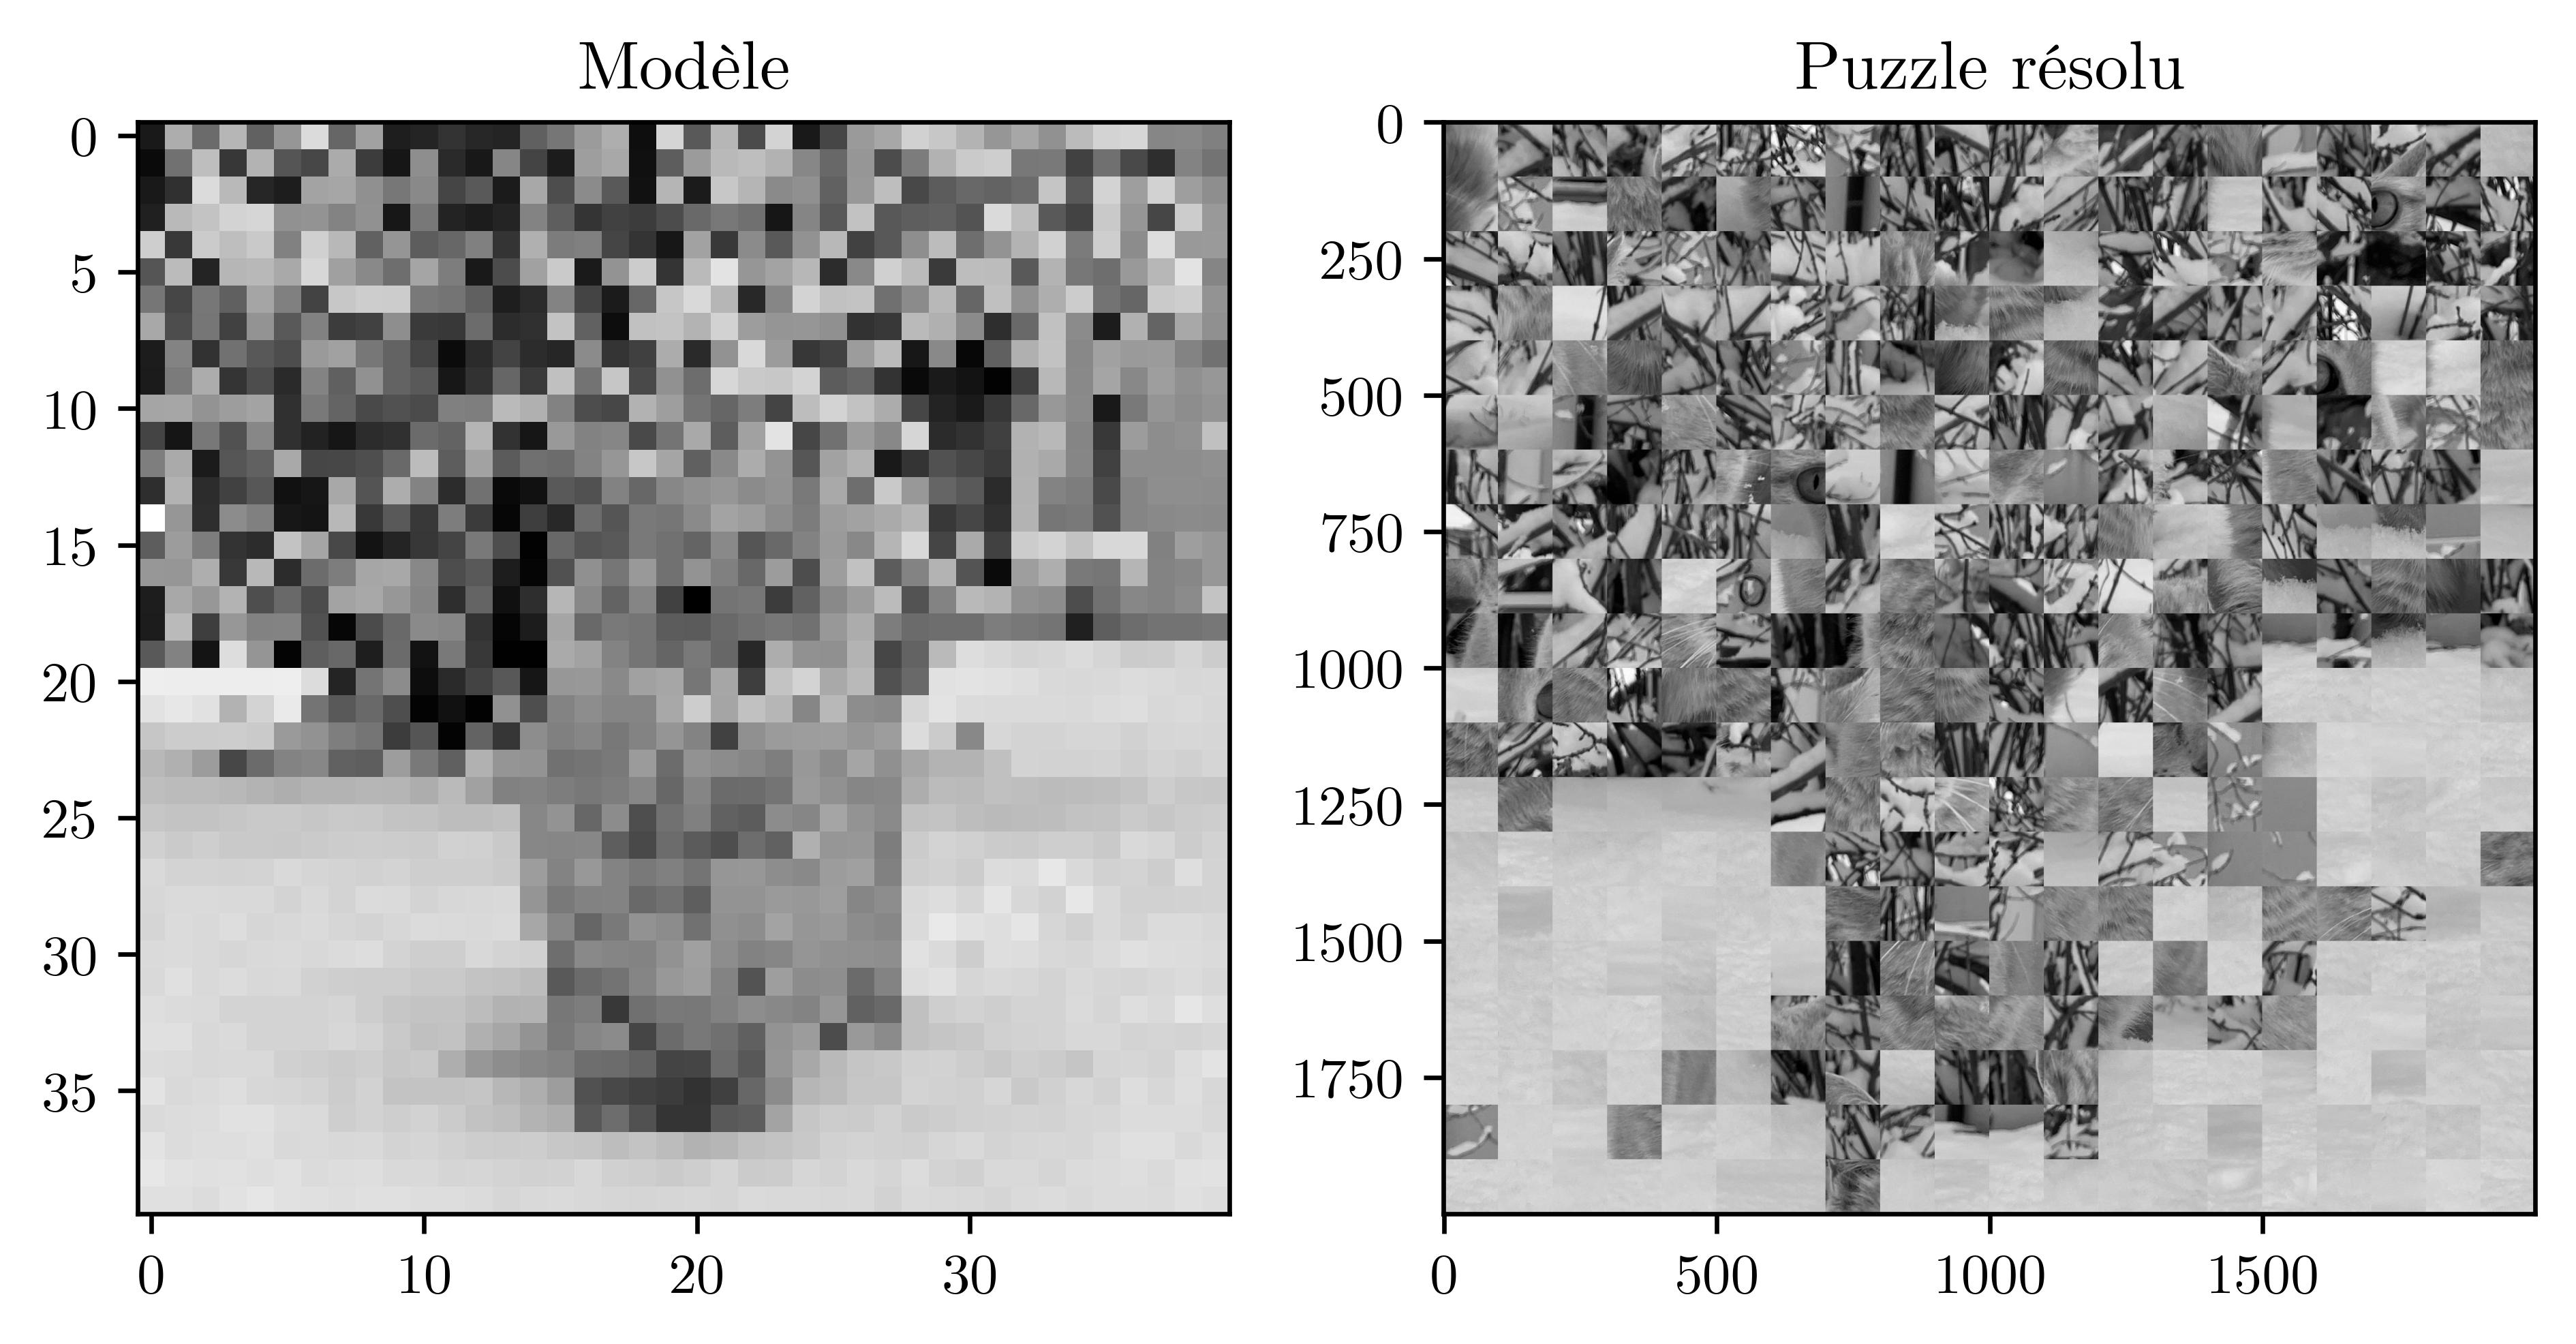
\includegraphics[width=\linewidth, height=0.8\textheight, keepaspectratio]{../Images/tigrou_erreur}
		\underline{Echec de résolution} (Taux de réduction: 50)
	\end{frame}

\end{document}